
\typeout{new file: Old_Species_RadCal_Chapter.tex}

\chapter{The Original RadCal Species}
\label{chap:old_species}

The characteristics of the original RadCal species, \textit{i.e.} the species present in the 1993 RadCal version, are presented in this chapter. These species are gas phase $\rm H_2O$, $\rm CO_2$, CO, and $\rm CH_4$. The data pertaining to these species have not been changed since the 1993 RadCal version.

\section{Water vapor: $\rm H_2O$}

The water molecule is an asymmetric top molecule with the oxygen atom in the middle. The bound length is 0.958 \AA{} and the bond angle is 104.45\textdegree. Because of its large permanent electric dipole moment ($6.16 \times 10^{-30}$ Coulomb-meters) in its equilibrium configuration, it has strong rotational bands. In addition, it three moments of inertia differ greatly: the rotational constants are A~=~27.877~cm$^{-1}$, B~=~14.512~cm$^{-1}$, and C~=~9.285~cm$^{-1}$ (values from Ref.~\cite{NIST2013}). Recall that the rotational constant relates to the molecule principal moment of inertia with:
\begin{equation}
 A = \dfrac{h}{8 \pi^2 c I_A},
\end{equation}
where $I_A$ is one of the principal moment of inertia, $h$ is the Planck constant ($6.626 \times 10^{-34}$~J$\cdot$s), and $c$ is the speed of light in vacuum, $c$ = $299,792,458$~m/s.

Because the three moments of inertia are greatly different from each other and are small, they give rise to a widespread and apparently disorderly array of rotation lines. This makes the infrared spectrum of $\rm H_2O$ very complex. $\rm H_2O$ has three fundamentals vibration modes, which are reported in Table \ref{table::fund_H2O}.

\begin{table}[ht]
    \centering
    \caption{Observed wavenumbers associated with fundamental vibration modes of $\rm H_2O$.}
    \label{table::fund_H2O}
    \begin{tabular}{|c|c|c|} \hline
    Band & Upper State & H$^{16}$OH  \\
    \hline
    $\nu_1$  &  100 & 3657.05 \\
    $\nu_2$  &  010 & 1594.75 \\
    $\nu_3$  &  001 & 3755.93 \\
    \hline
   \end{tabular}
\end{table}

The important bands of water vapor fall into a number of distinct classes: rotation band from 0 to 900~cm$^{-1}$, $\nu_2$ bands from 900 to 2400~cm$^{-1}$ (6.3 $\rm \mu m$ region), $\nu_1$, $\nu_3$, and 2$\nu_2$ bands from 2800 to 4400~cm$^{-1}$ (2.7 $\rm \mu m$ region), 6 distinguishable groups of lines between 4500 and 11,000~cm$^{-1}$: $\Omega$, $\Psi$, $\Phi$, $\tau^c$, $\sigma^c$, $\rho^c$; these are combined vibrational modes and overtones.

The strongest bands at atmospheric temperature are the rotational (0 -- 900~cm$^{-1}$) and the 6.3~$\rm \mu m$ band. In fire application, the shift of the dominant region of the Planck distribution toward higher wavenumber renders the 2.7~$\mu$m very important for high temperature emission purposes.

In Radcal, the $\rm H_2O$ mean absorption coefficient $\bar{\kappa}$ has been tabulated for the wavenumbers between 50 to 9300~cm$^{-1}$, and for the following temperatures: 300~K, 600~K, 1000~K, 1500~K, 2000~K, 2500~K. Figure~\ref{fig:H2O_300-2500K} displays the spectral mean absorption coefficient, in units of $\rm atm^{-1}.cm^{-1}$, at these different temperatures. The data originate from Ludwig \textit{et al.}~\cite{Ludwig1973}. Experimental data have been fitted using the statistical Goody narrow band model.

\begin{figure}[p]
\begin{tabular*}{\textwidth}{l@{\extracolsep{\fill}}r}
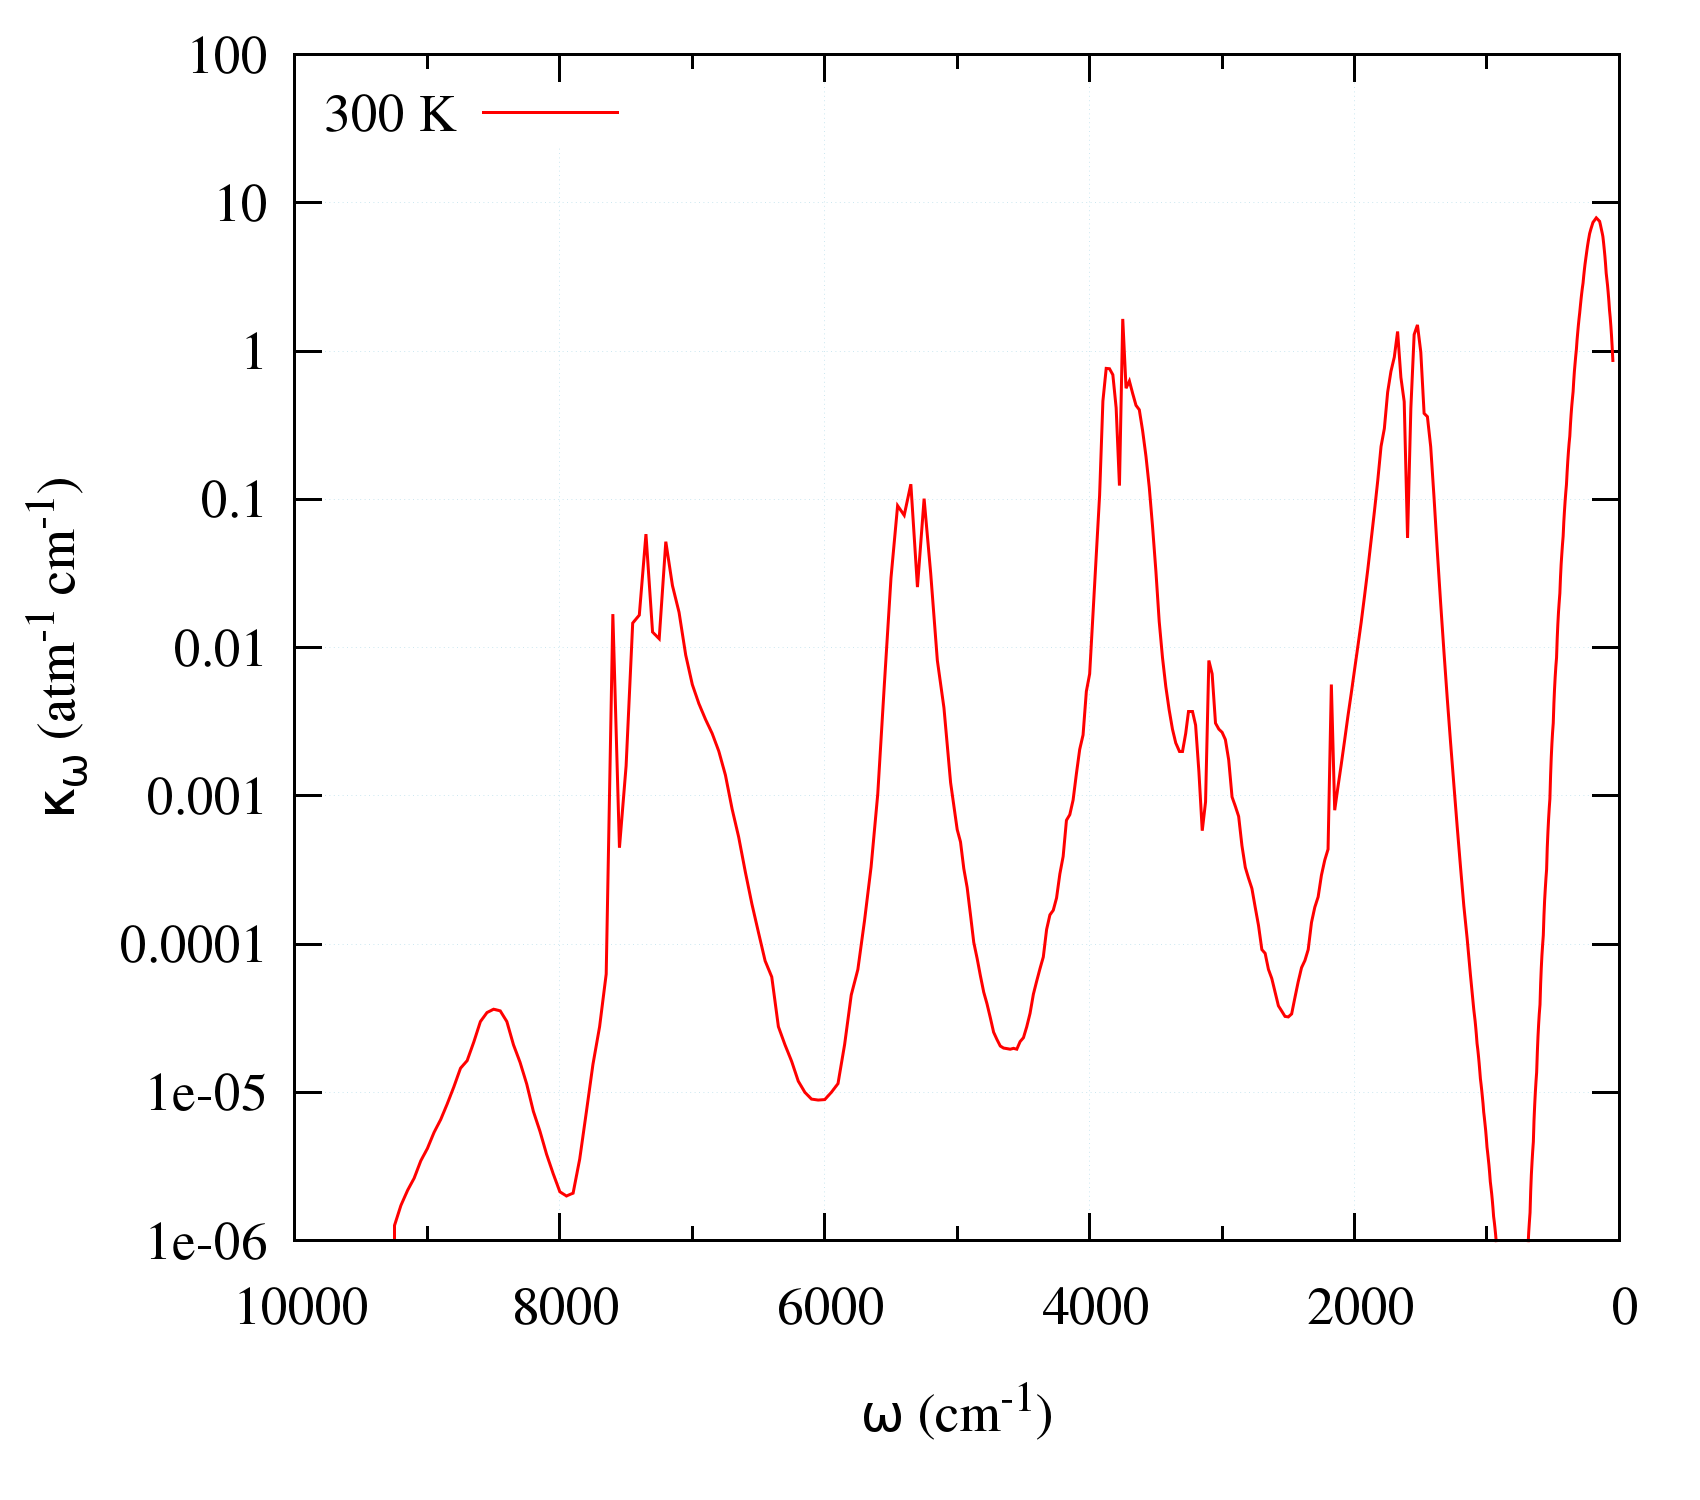
\includegraphics[height=2.5in]{Figures/H2O_300K.png} &
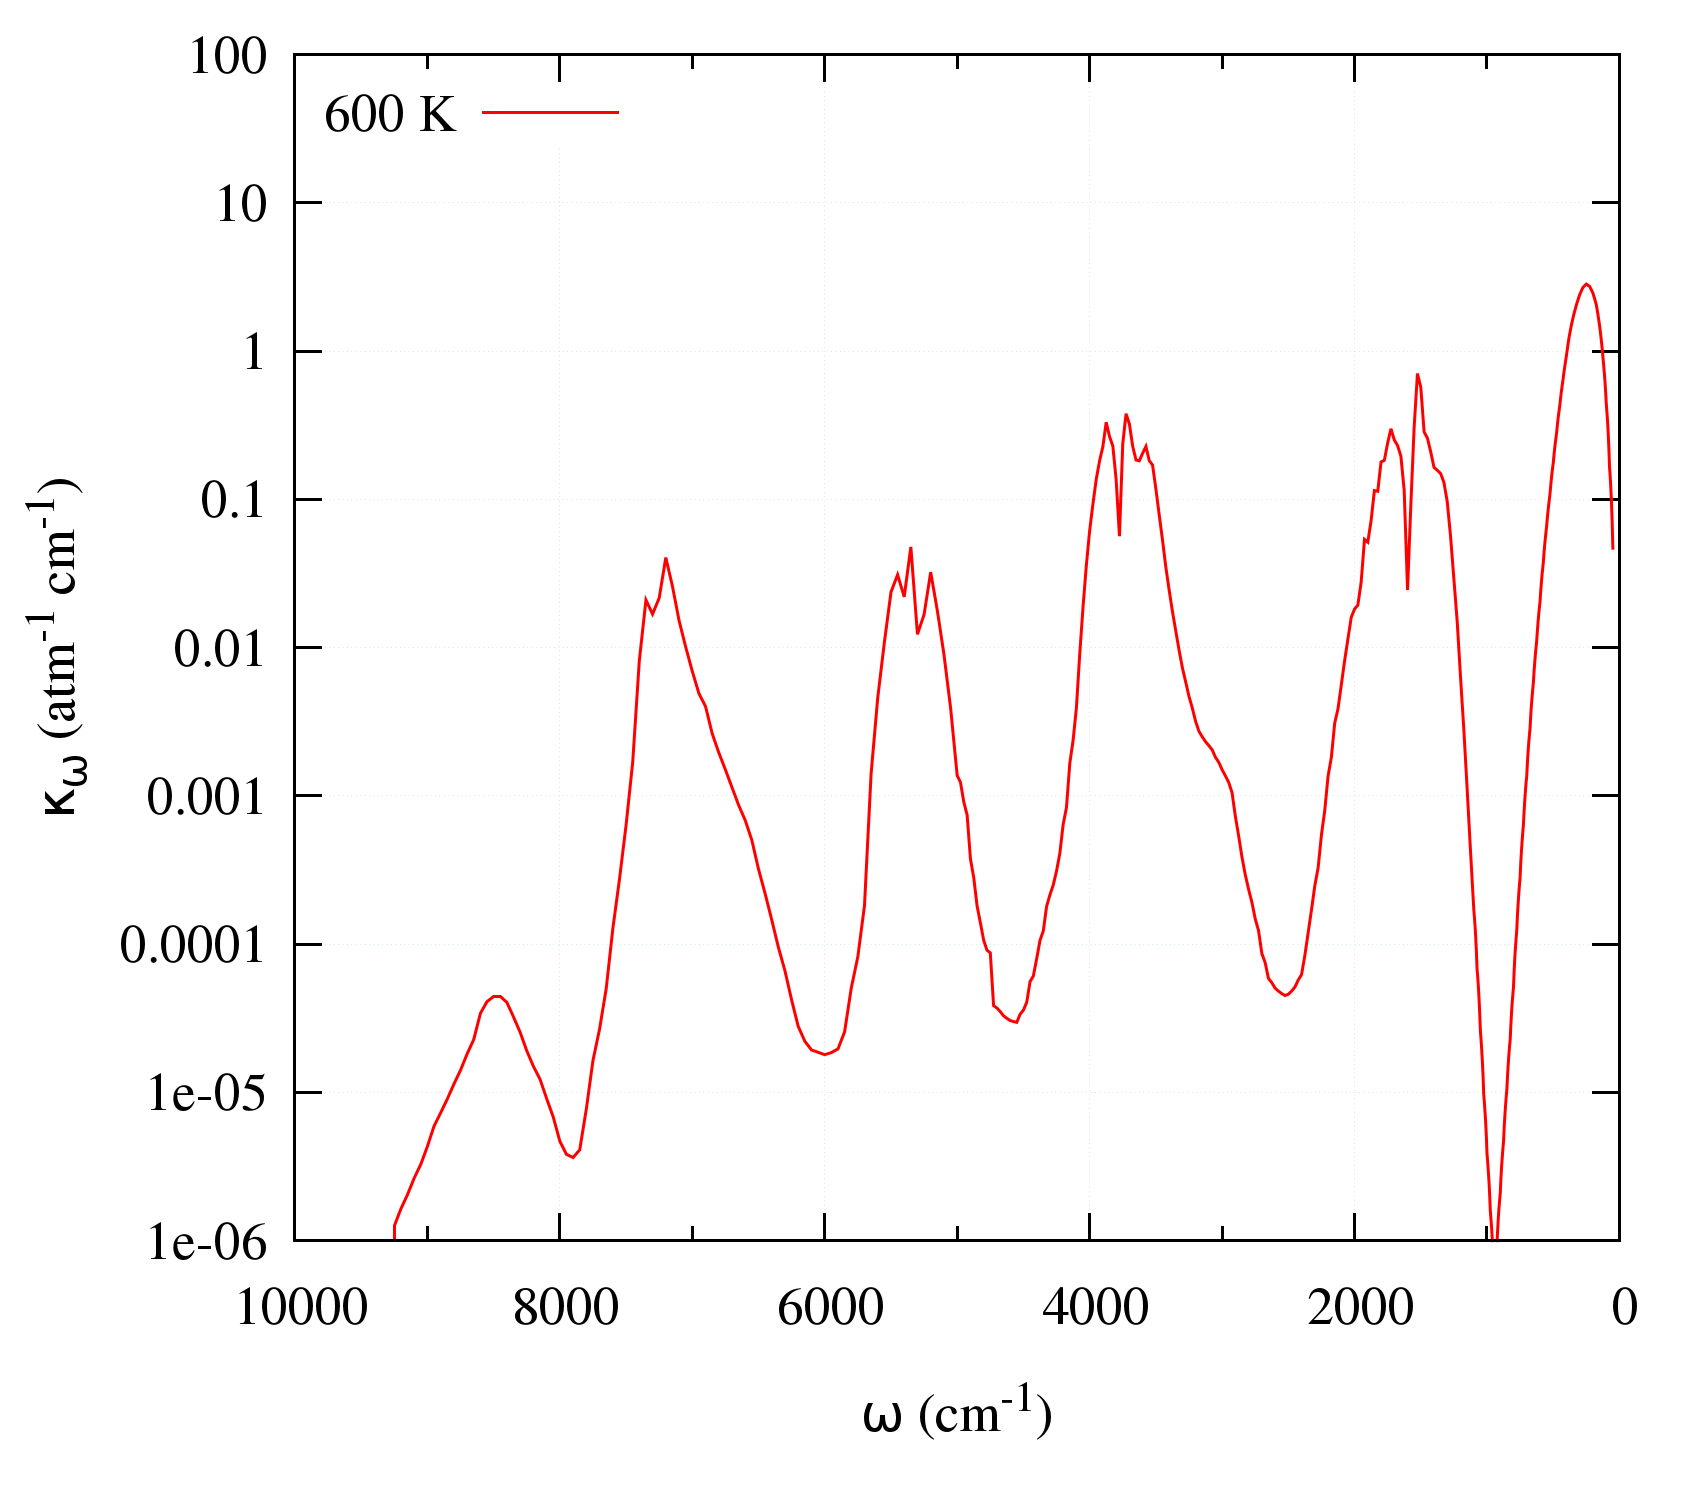
\includegraphics[height=2.5in]{Figures/H2O_600K.png} \\
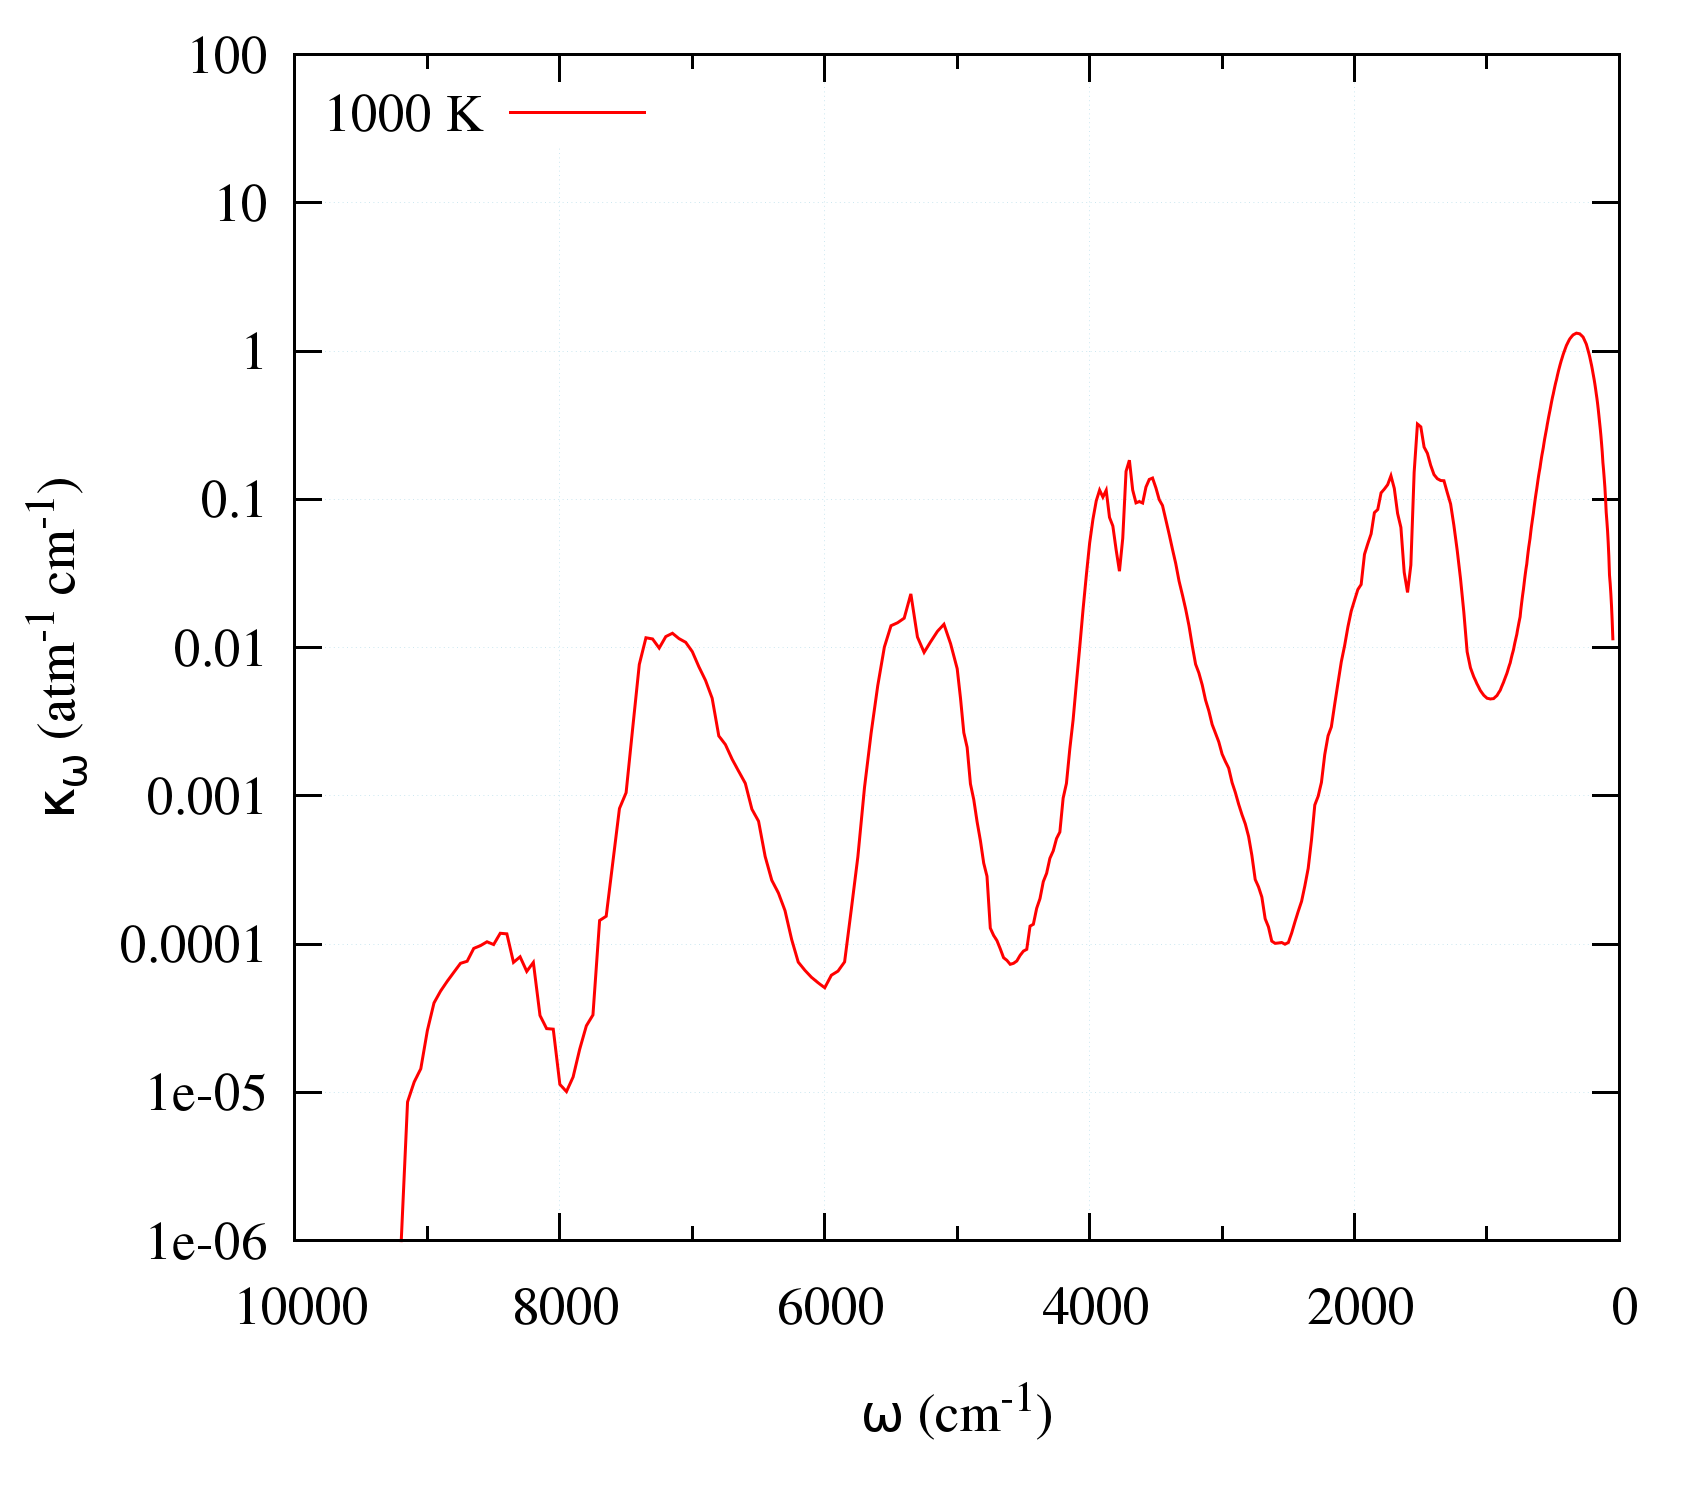
\includegraphics[height=2.5in]{Figures/H2O_1000K.png} &
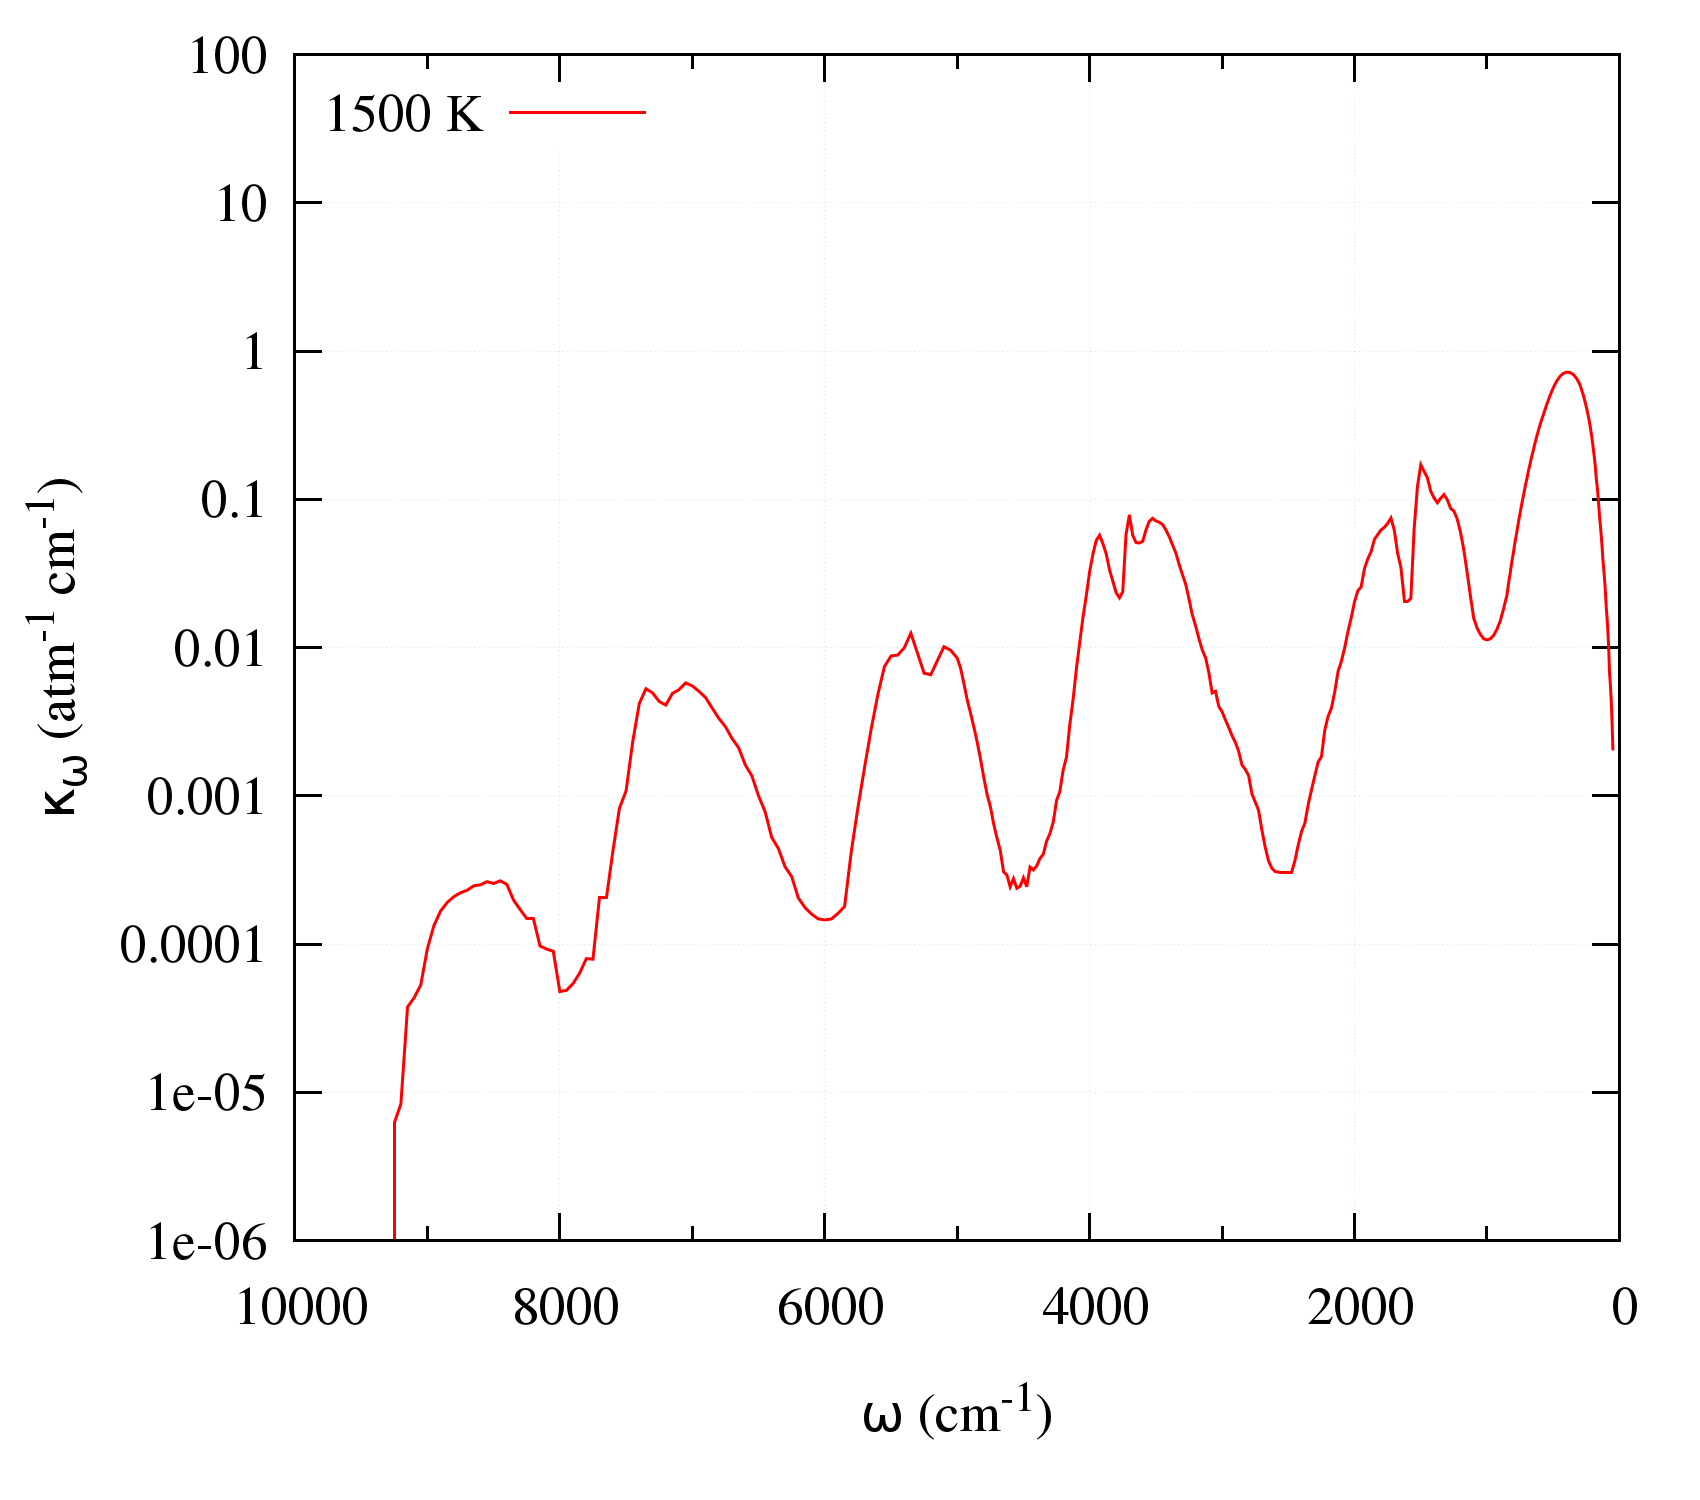
\includegraphics[height=2.5in]{Figures/H2O_1500K.png} \\
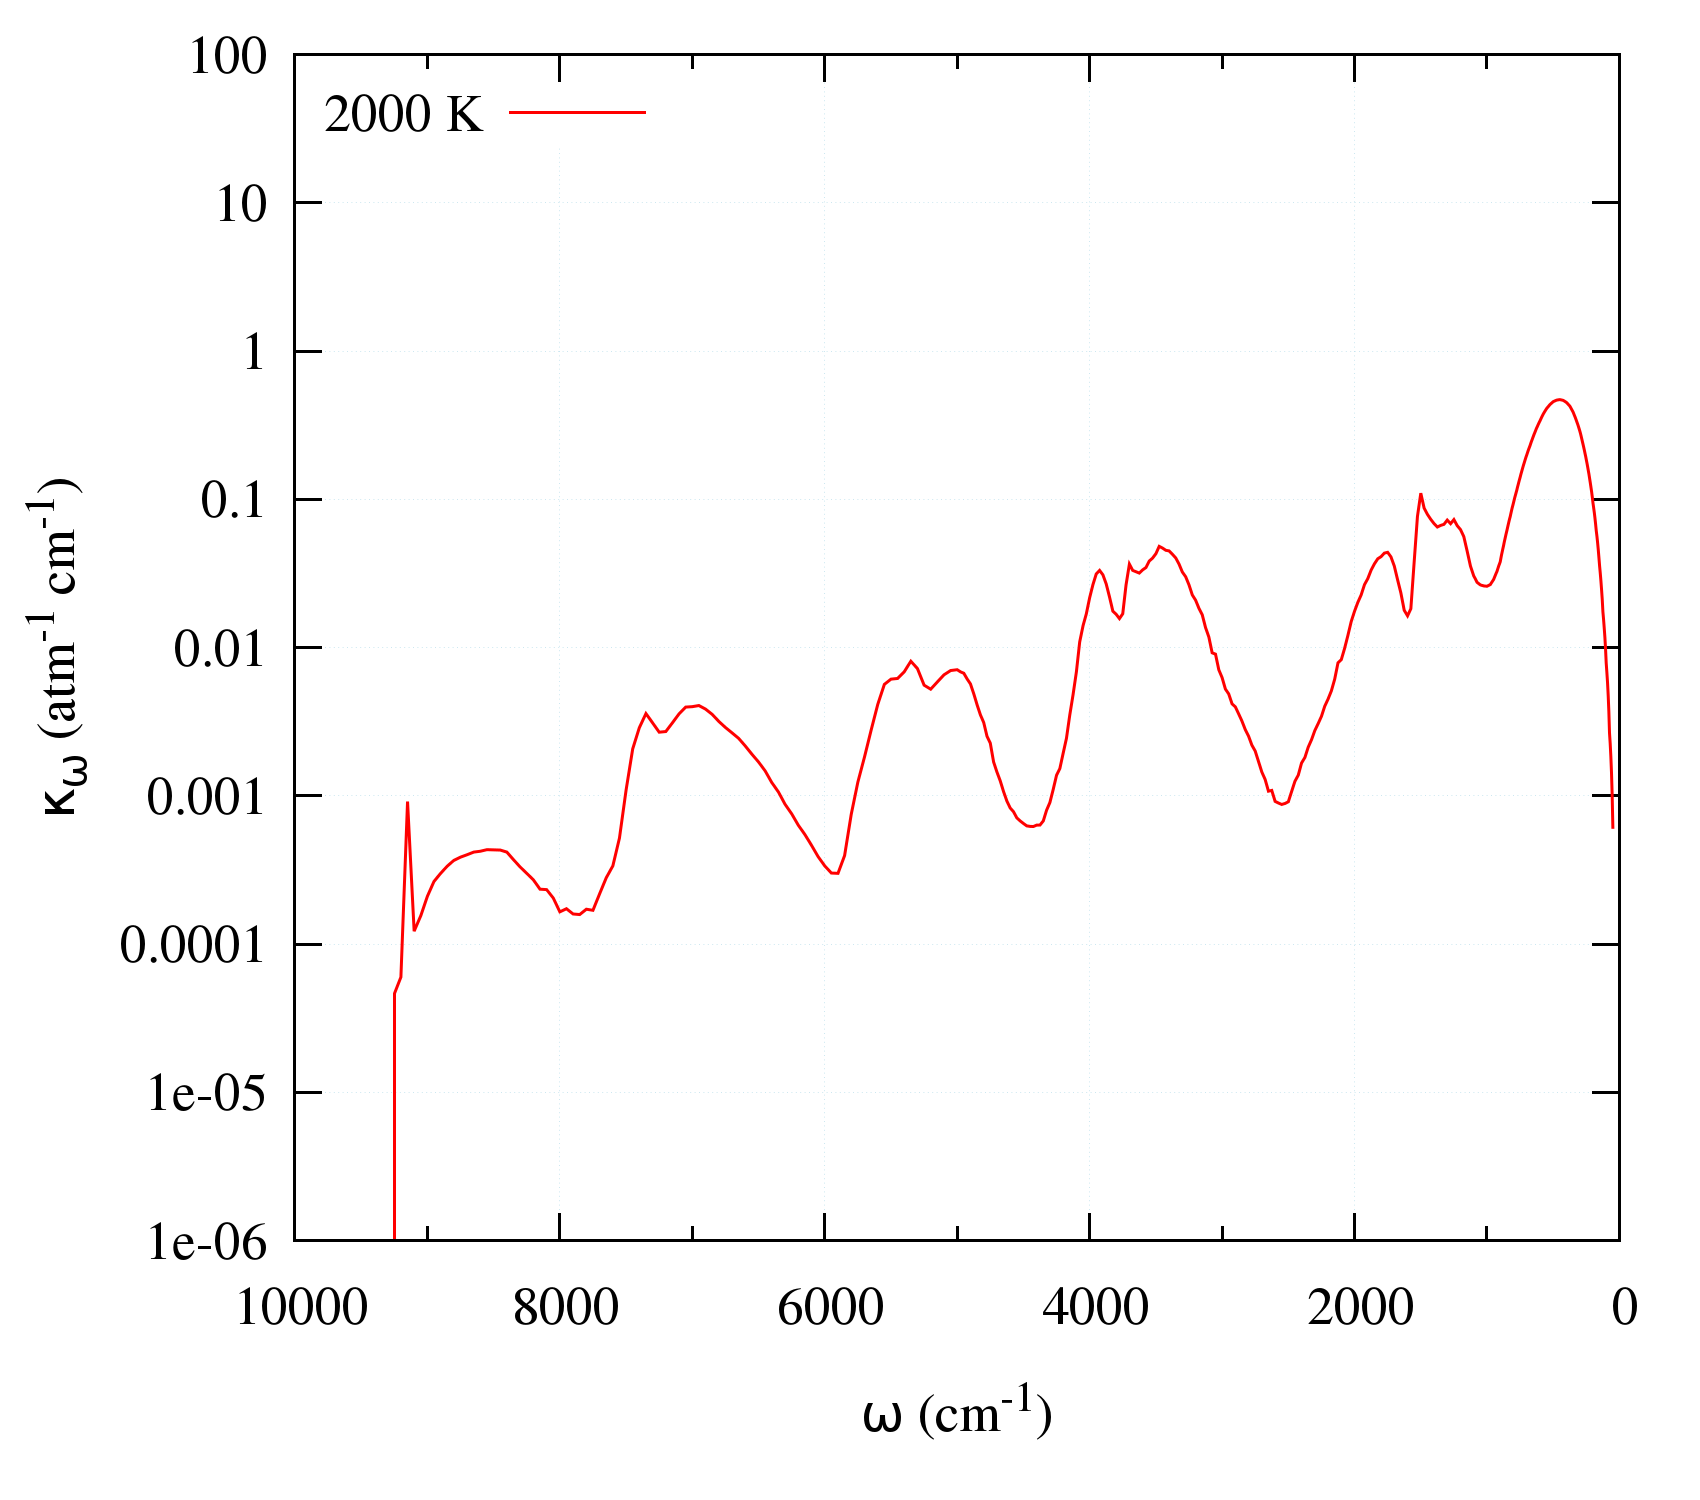
\includegraphics[height=2.5in]{Figures/H2O_2000K.png} &
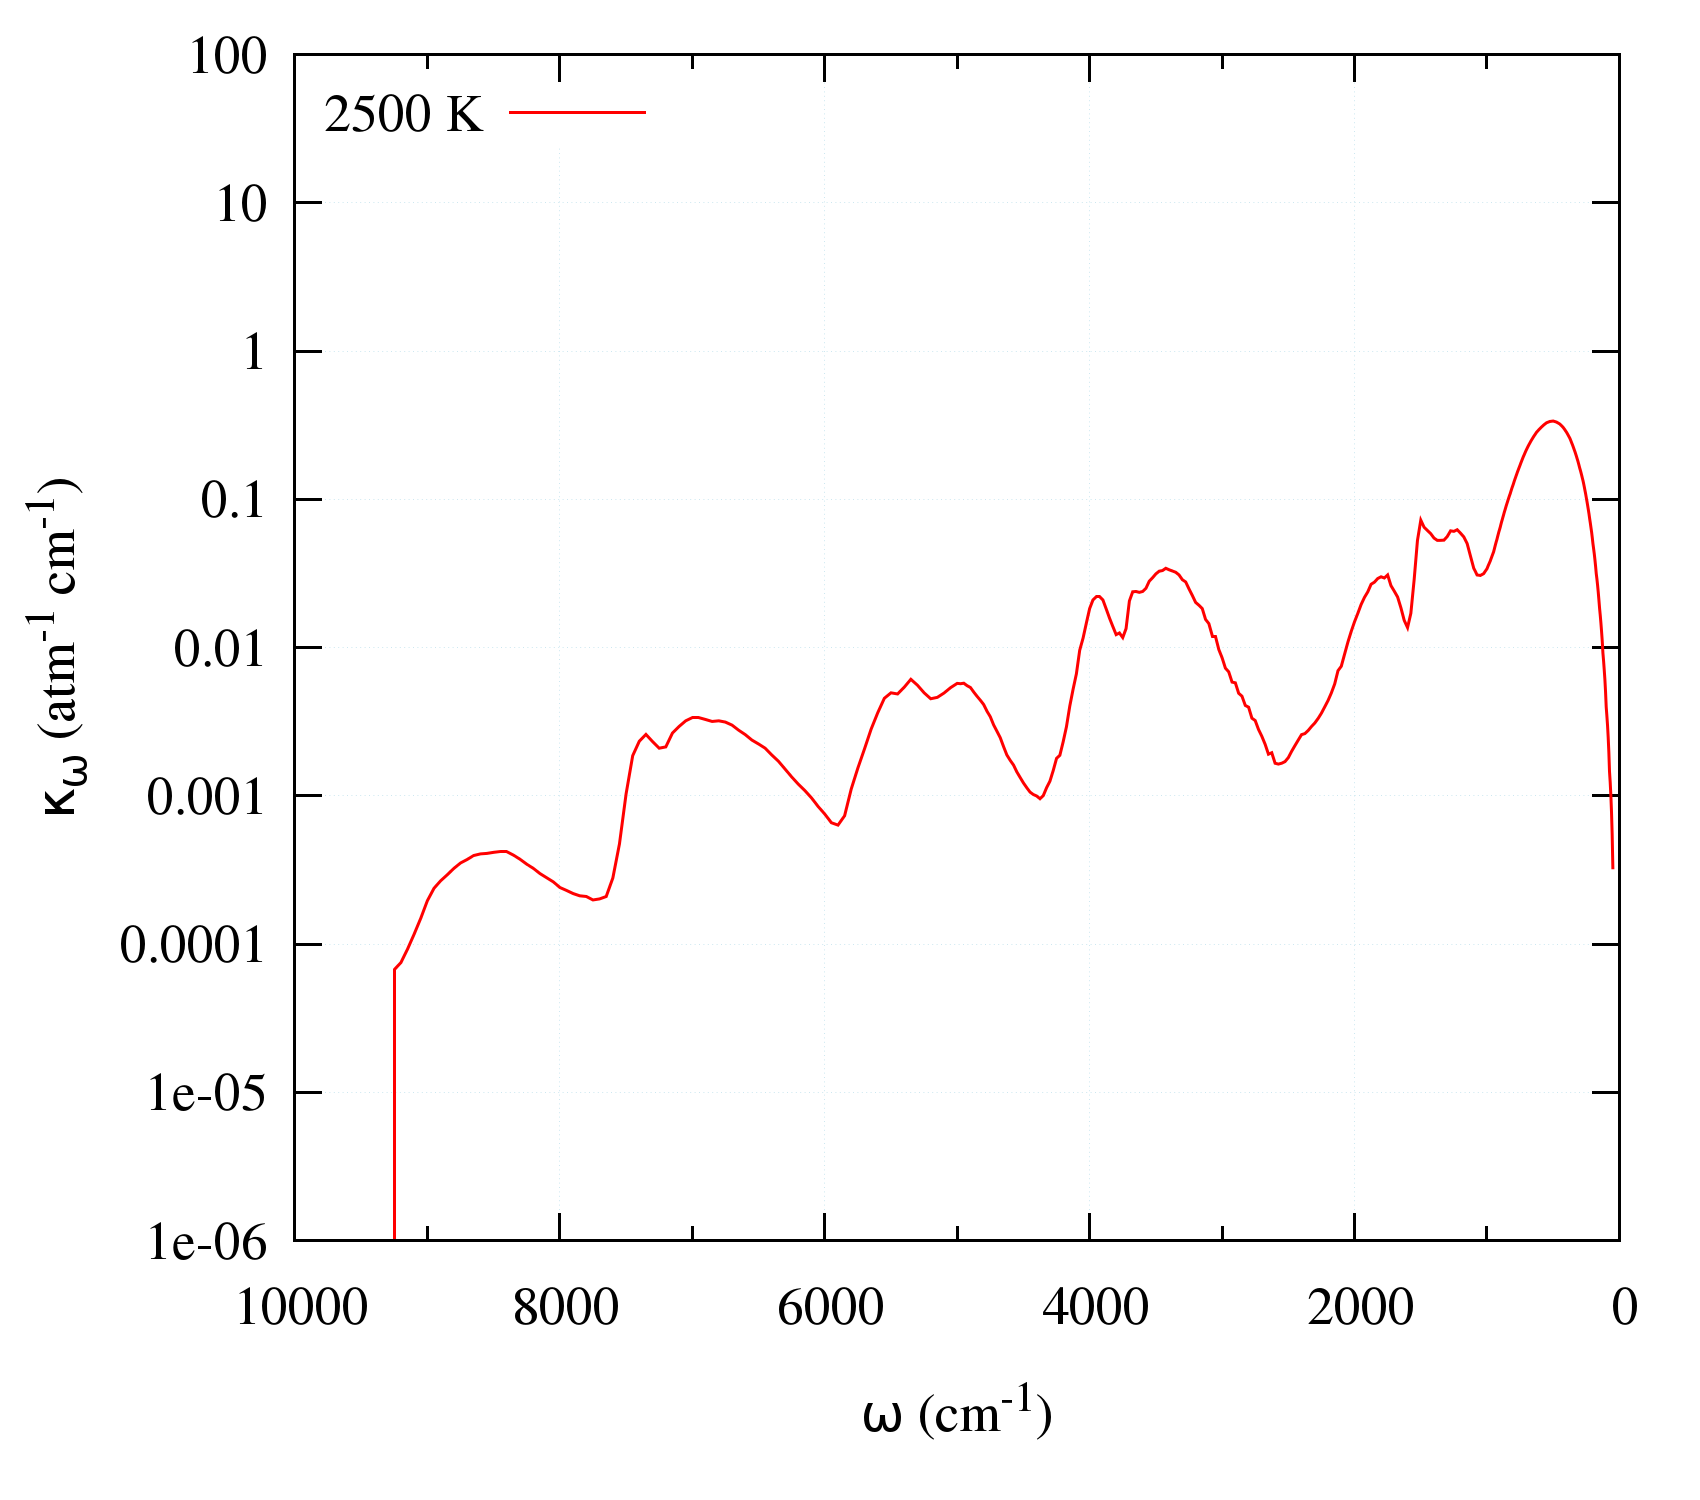
\includegraphics[height=2.5in]{Figures/H2O_2500K.png}
\end{tabular*}
\caption{Spectral variations of the $\rm H_2O$ mean absorption coefficient $\bar{\kappa}_{\om}$, in $\rm atm^{-1}.cm^{-1}$, at various temperatures as tabulated in RadCal.\label{fig:H2O_300-2500K}}
\end{figure}

To calculate the band overlap parameter $\beta$, the Lorentz HWHM is considered constant over the spectrum and is calculated using Eq.~\ref{eq:gamma_L}, while the effective line spacing is given by \cite{Ludwig1973}:
\begin{equation}
 d = \exp\left(0.7941 \sin\left(0.036 \omega- 8.043\right) + 2.294 + 0.3004 \times 10^{-2} T - 0.366 \times 10^{-6} T^2\right),
\end{equation}
where $T$ is the local temperature.


\clearpage

\section{Carbon dioxide: $\rm CO_2$}

Carbon dioxide is a linear, symmetric molecule. Its bond length is 115.98~pm in ground state, and its rotational constant is 0.3906~cm$^{-1}$. Because of the symmetry, $\rm CO_2$ has no permanent dipole moment. It has four vibrational modes, but only two fundamental IR vibration modes. Five distinct bands are included in RadCal (four are calculated, one is tabulated), see Table \ref{Table::CO2}. All the bands are modeled after the Goody model.

\begin{table}[h!]
    \centering
    \caption{Spectral bands of $\rm CO_2$ included in RadCal.}
    \label{Table::CO2}
    \begin{tabular}{|c|c|c|c|l|}
      \hline
      Band \# & \multicolumn{2}{|l|}{Bounds (cm$\rm ^{-1}$) } & Method & Notes: \\
      \cline{1-5}
      1 &  500 & 880  & tabulated&  15 $\mu$m region - strong (for atmospheric application)\\
      2 &  880 & 1100 & modeled  & 10 $\mu$m region\\
      3 & 1975 & 2475 & modeled  & 4.9 and 4.3 $\mu$m region - very strong\\
      4 & 3050 & 3800 & modeled  & 2.7 $\mu$m region - important for fire application\\
      5 & 4550 & 5275 & modeled  & 2.0 $\mu$m region\\
      \hline
    \end{tabular}
\end{table}

\begin{figure}[p]
\begin{tabular*}{\textwidth}{l@{\extracolsep{\fill}}r}
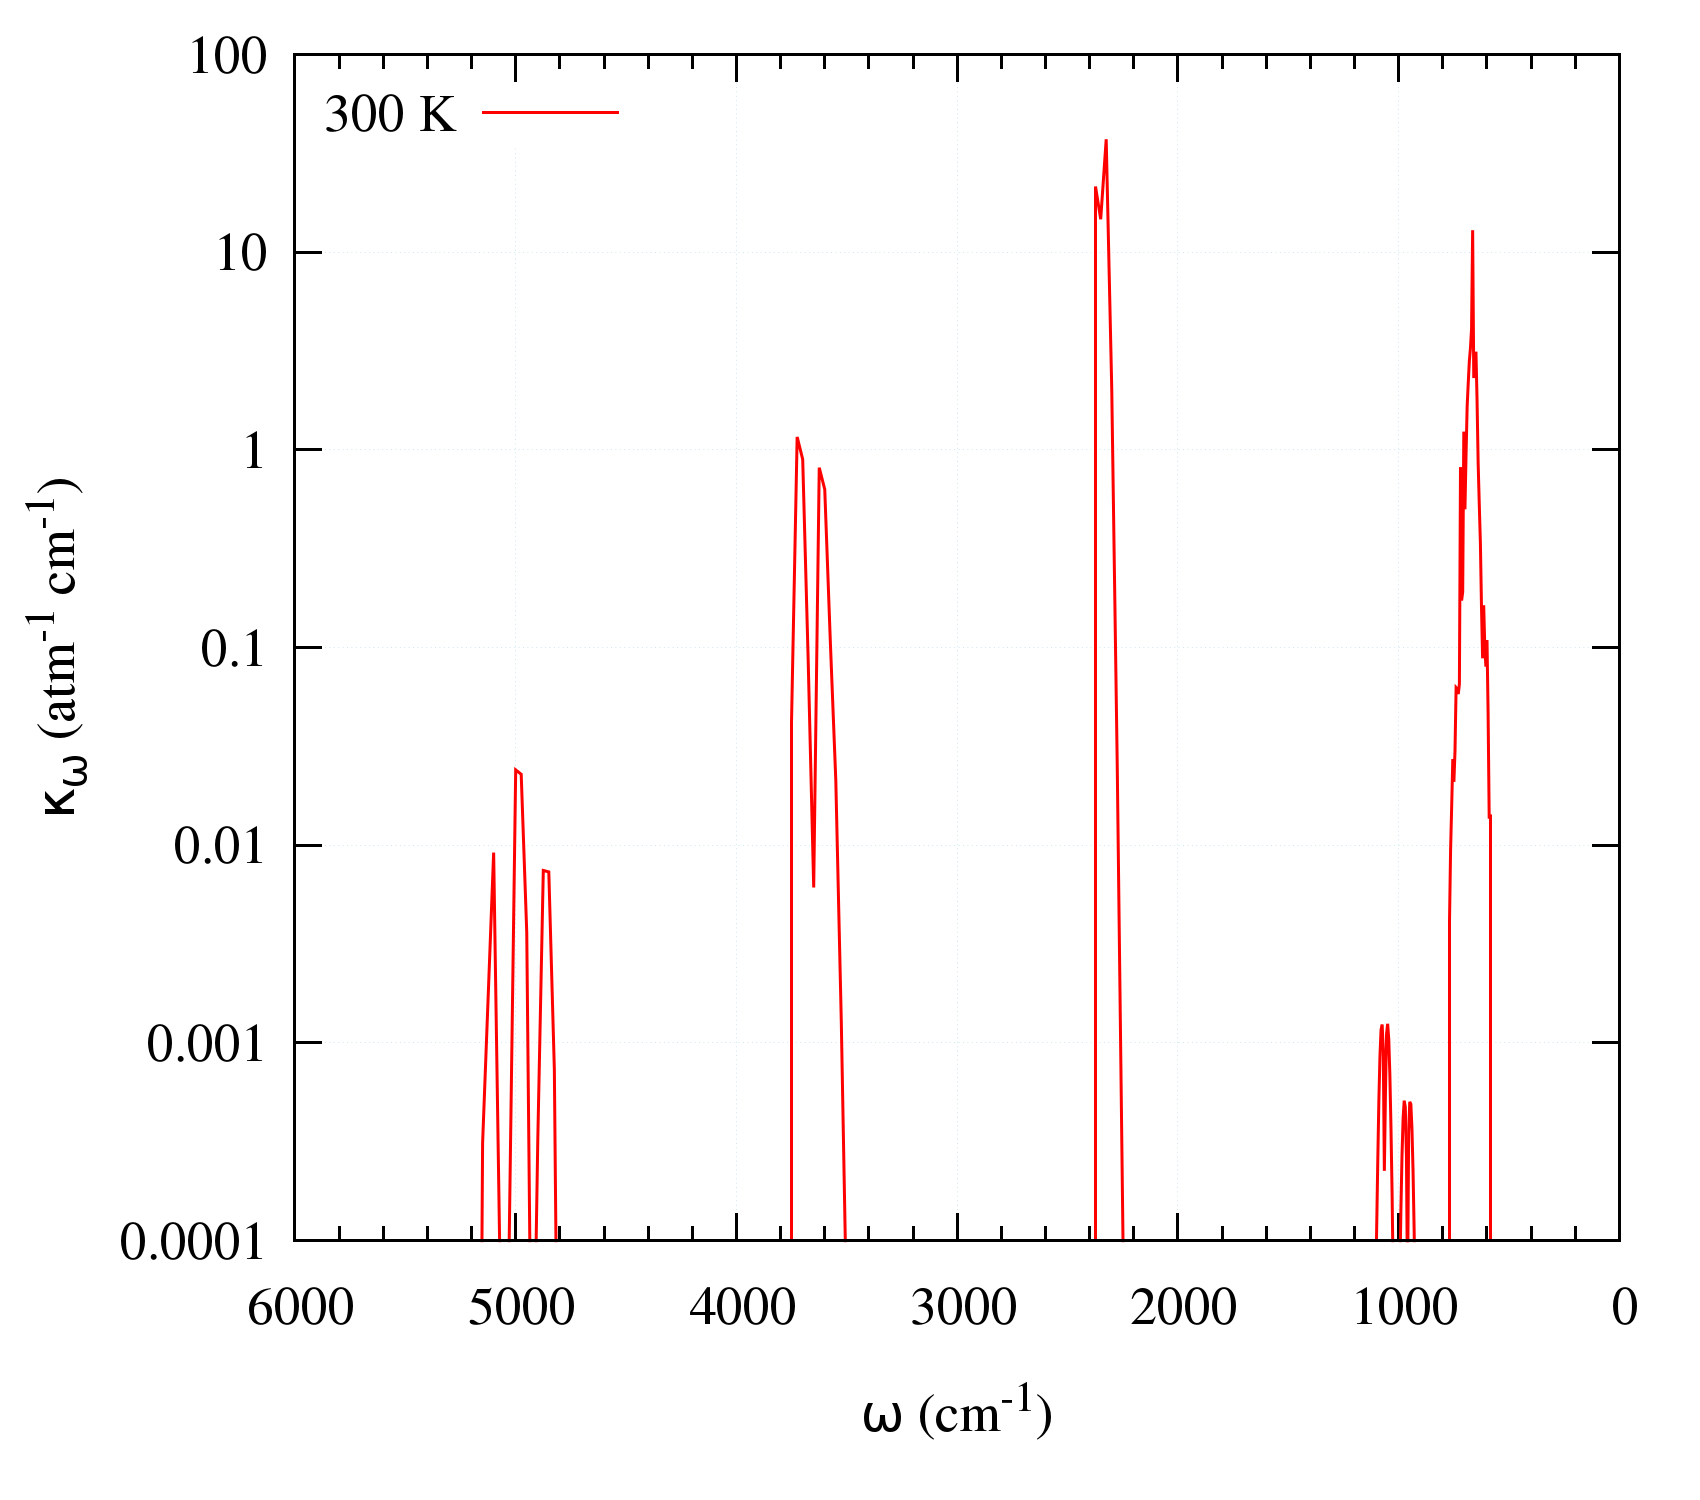
\includegraphics[height=2.5in]{Figures/CO2_300K.png} &
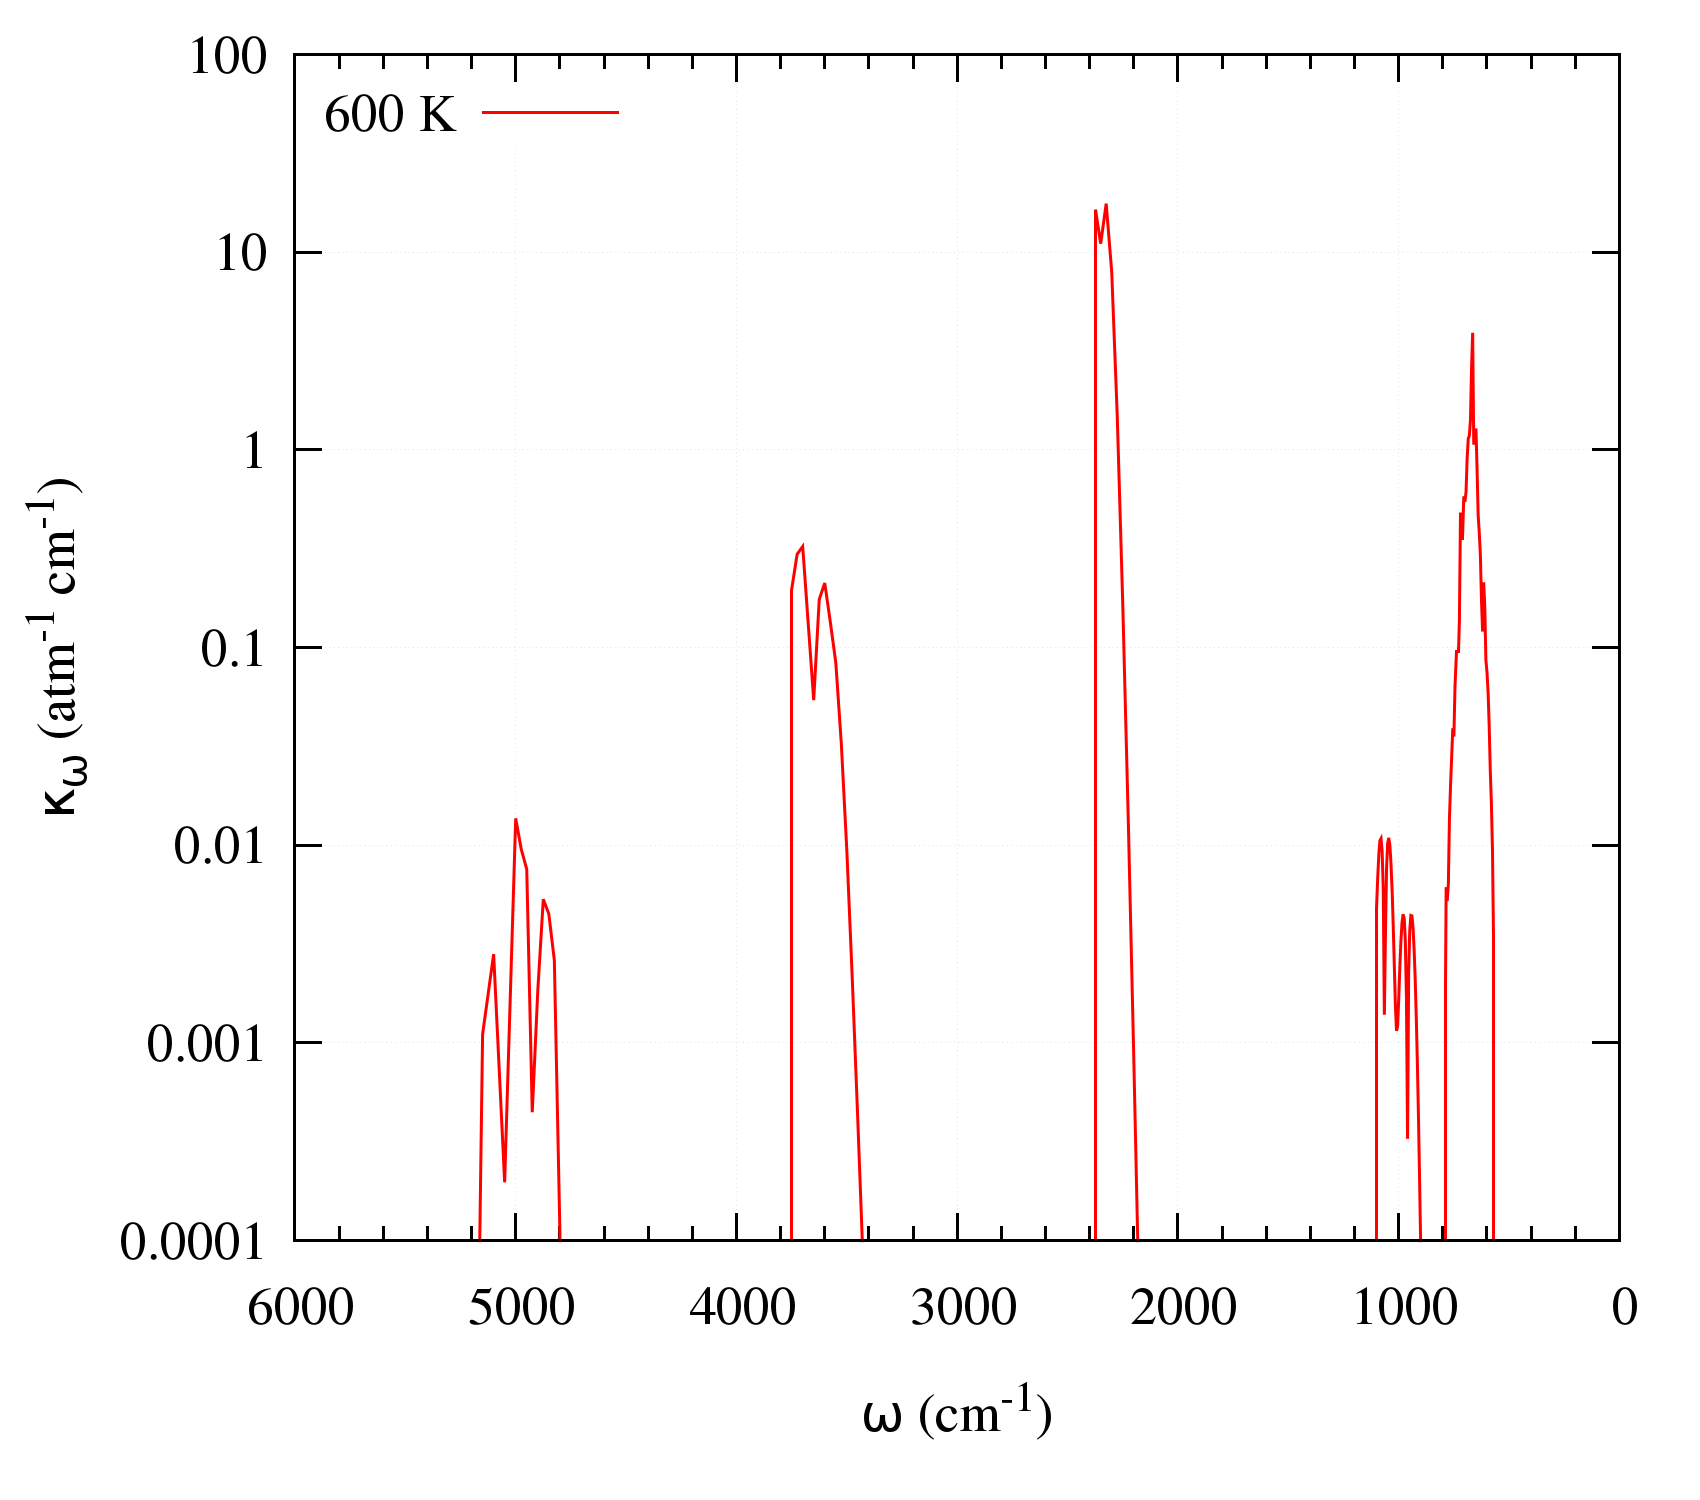
\includegraphics[height=2.5in]{Figures/CO2_600K.png} \\
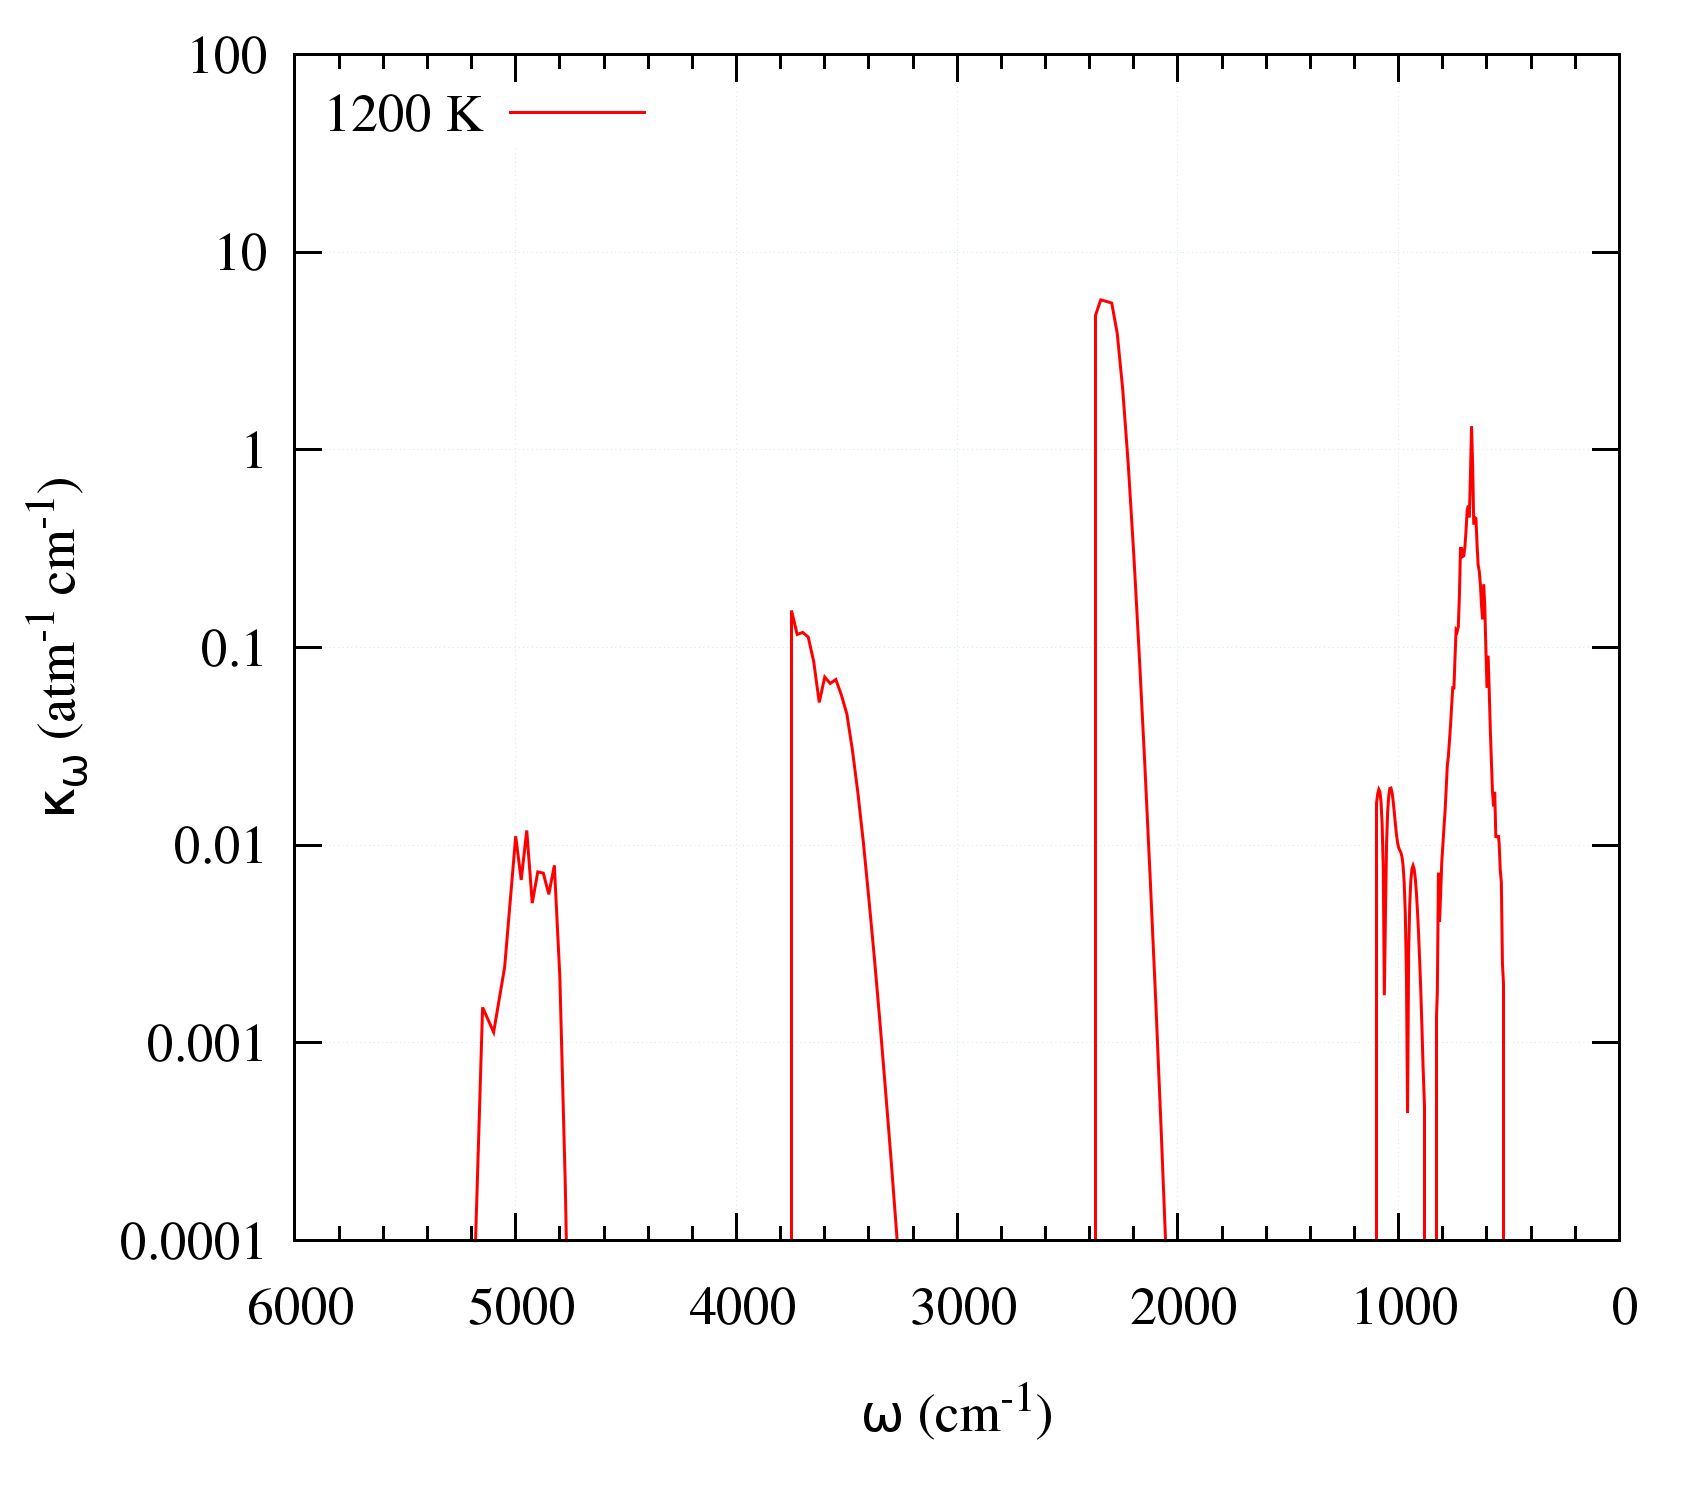
\includegraphics[height=2.5in]{Figures/CO2_1200K.png} &
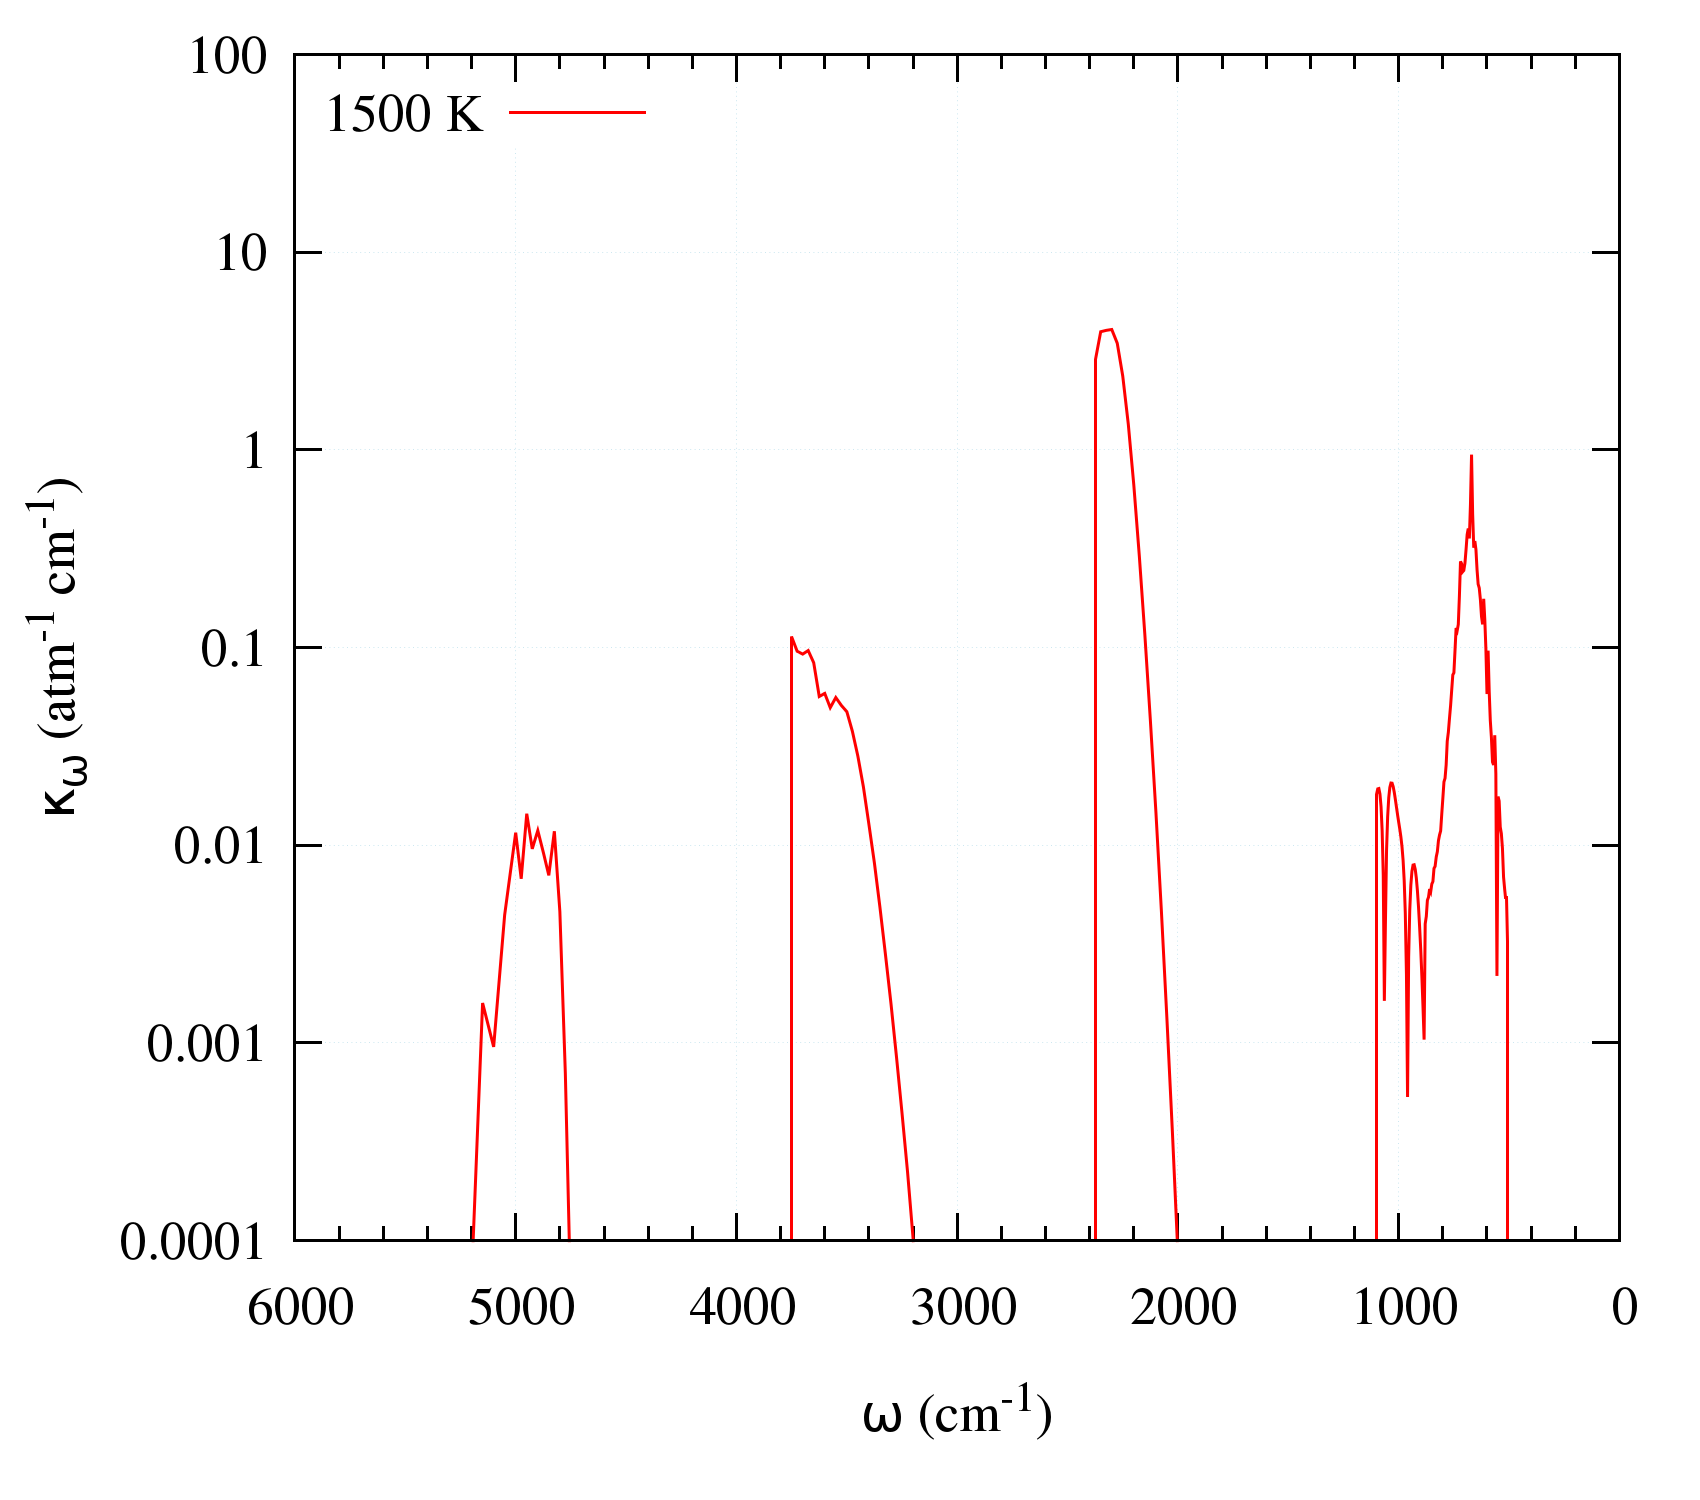
\includegraphics[height=2.5in]{Figures/CO2_1500K.png} \\
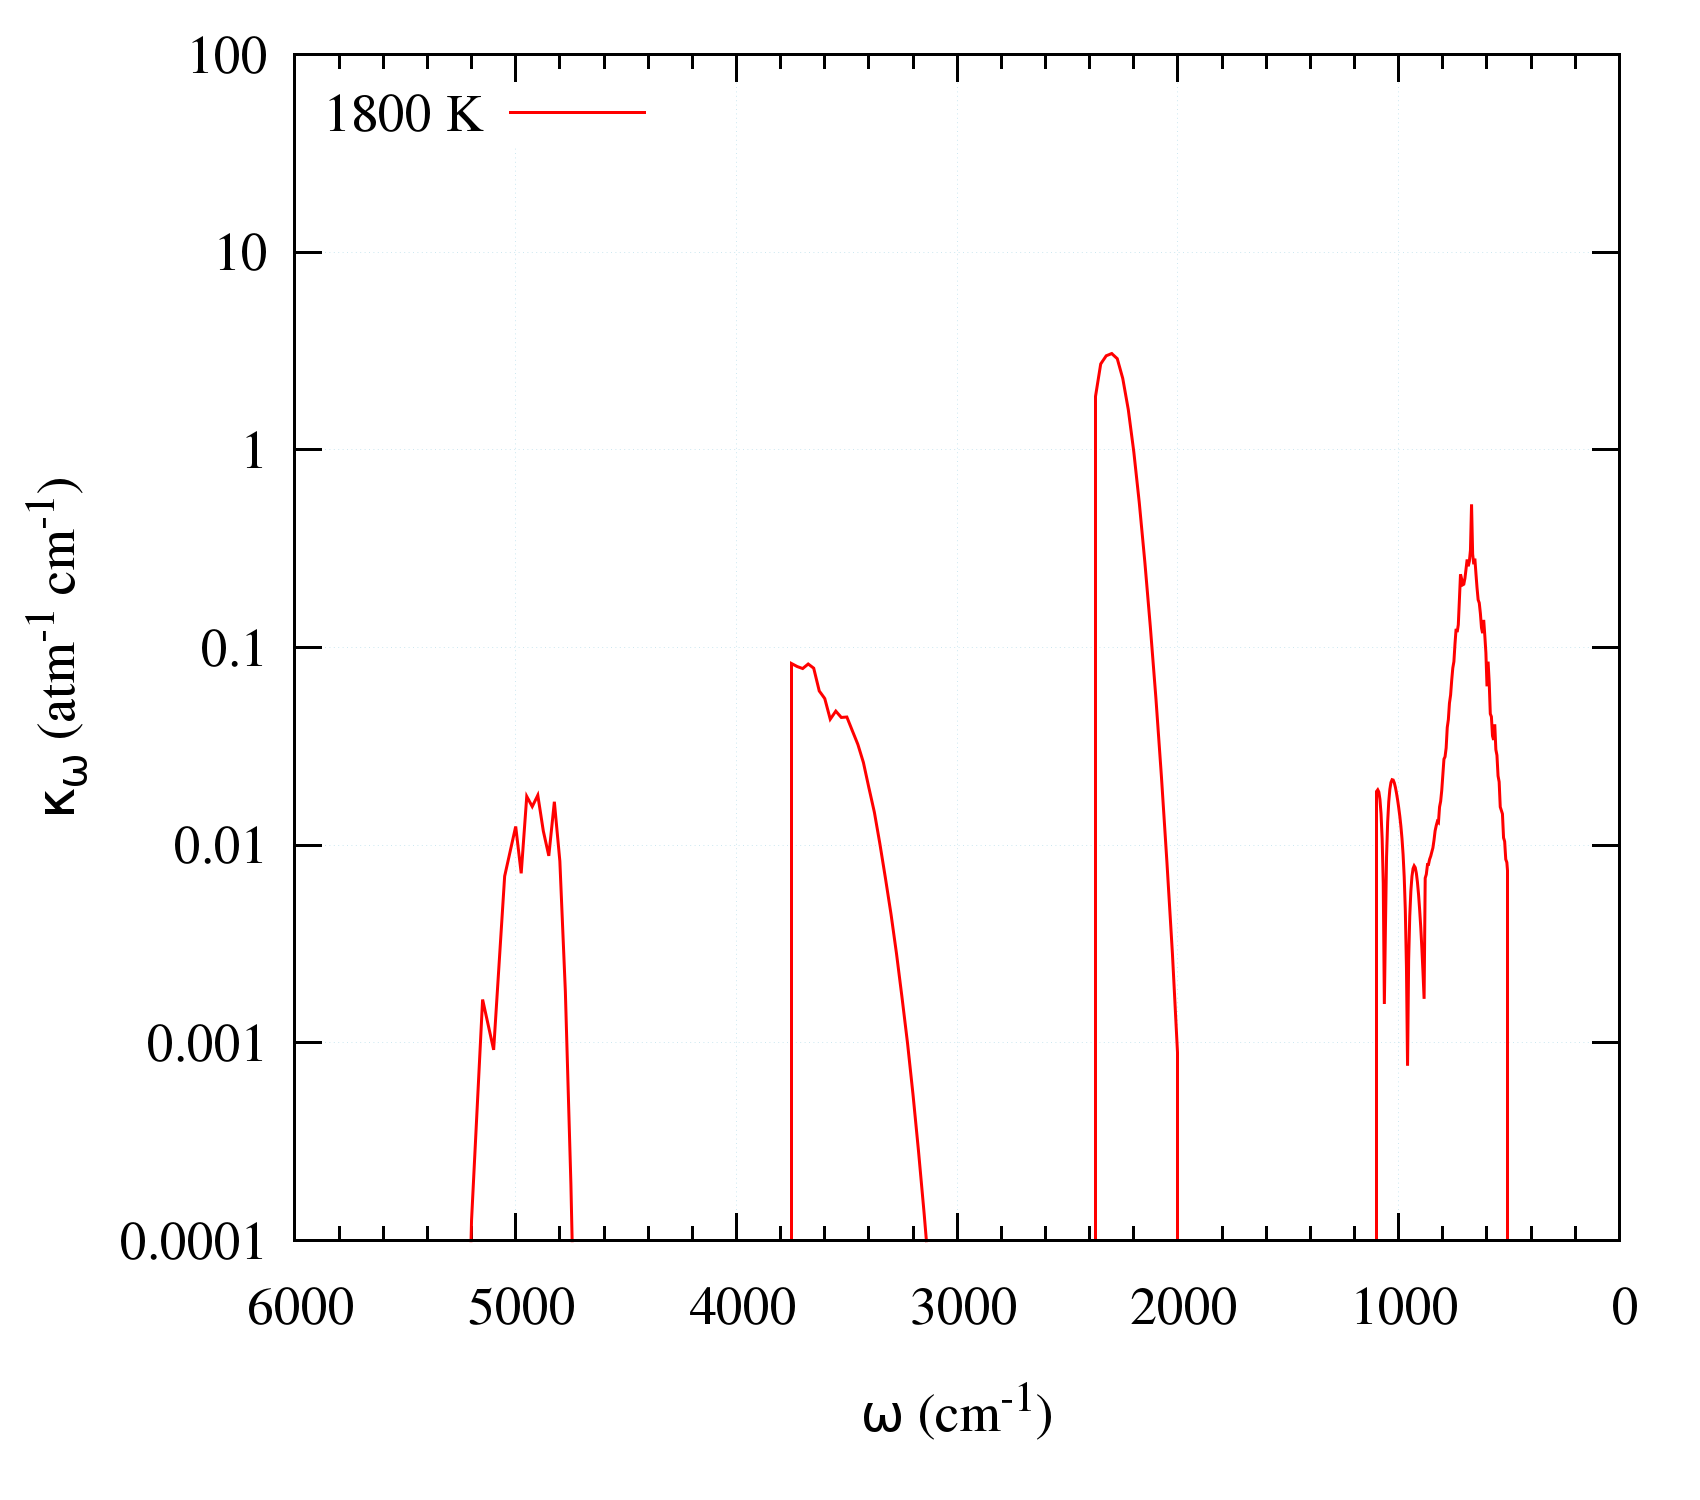
\includegraphics[height=2.5in]{Figures/CO2_1800K.png} &
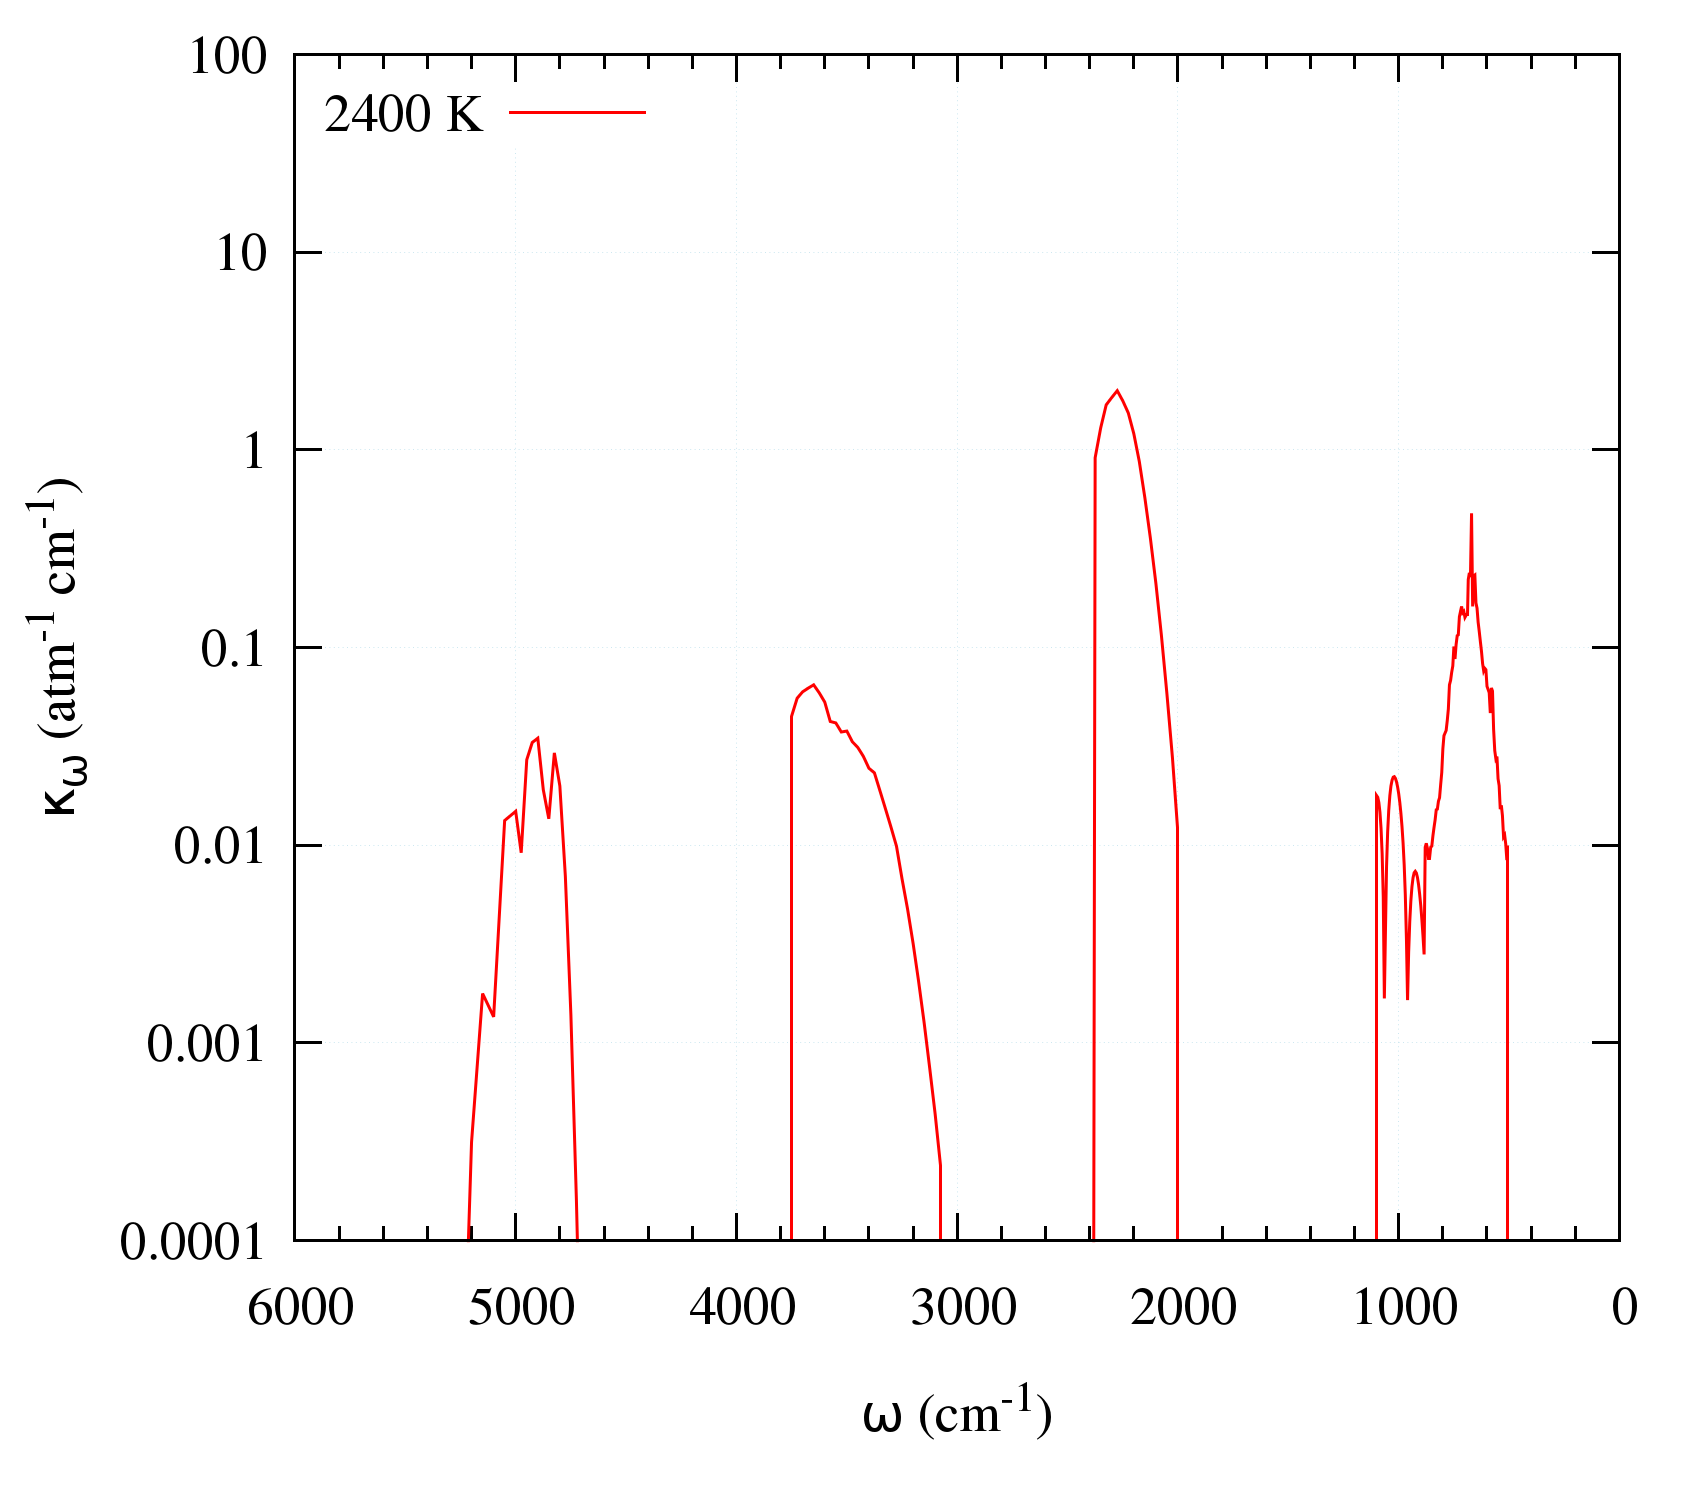
\includegraphics[height=2.5in]{Figures/CO2_2400K.png}
\end{tabular*}
\caption{Spectral variations of the $\rm CO_2$ mean absorption coefficient $\bar{\kappa}_{\om}$, in $\rm atm^{-1}.cm^{-1}$, at various temperatures as tabulated in RadCal.\label{fig:CO2_300-2500K}}
\end{figure}

The strongest band in the $\rm CO_2$ spectrum is Band~3. At 300~K, it has an integrated band intensity (see Section~\ref{sec:integrated_intensity} for a definition of this quantity) of 2963~atm$^{-1}$cm$^{-2}$. The tabulated data (mean absorption coefficient $\bar{\kappa}_{\om}$) were obtained from experiments for the following temperatures: 300, 600, 1200, 1500, 1800, 2400~K. The modeled bands use the harmonic oscillator approximation. All the bands uses the Goody statistical narrow band model. Figure~\ref{fig:CO2_300-2500K} to displays the mean absorption coefficient at 300, 600, 1200, 1500, 1800, 2400~K, as tabulated (Band 1) and modeled in RadCal (Bands 2 to 5).


\clearpage

\section{Carbon monoxide: $\rm CO$}

Carbon Monoxide is a diatomic molecule and as such, it has only one fundamental vibrational mode. RadCal includes one distinct band, the 1600--2400 band. It corresponds to the stretching of the triple bond $\rm C \equiv O$. This band is modeled and it uses the model from Malkmus and Thompson \cite{Malkmus1962}. It is based on the anharmonic oscillator model and uses band integrated intensity measurements. Figure~\ref{fig:CO_300-2500K} displays the spectral mean absorption coefficient of CO at 300~K and 2500~K.

\begin{figure}[ht]
\begin{tabular*}{\textwidth}{l@{\extracolsep{\fill}}r}
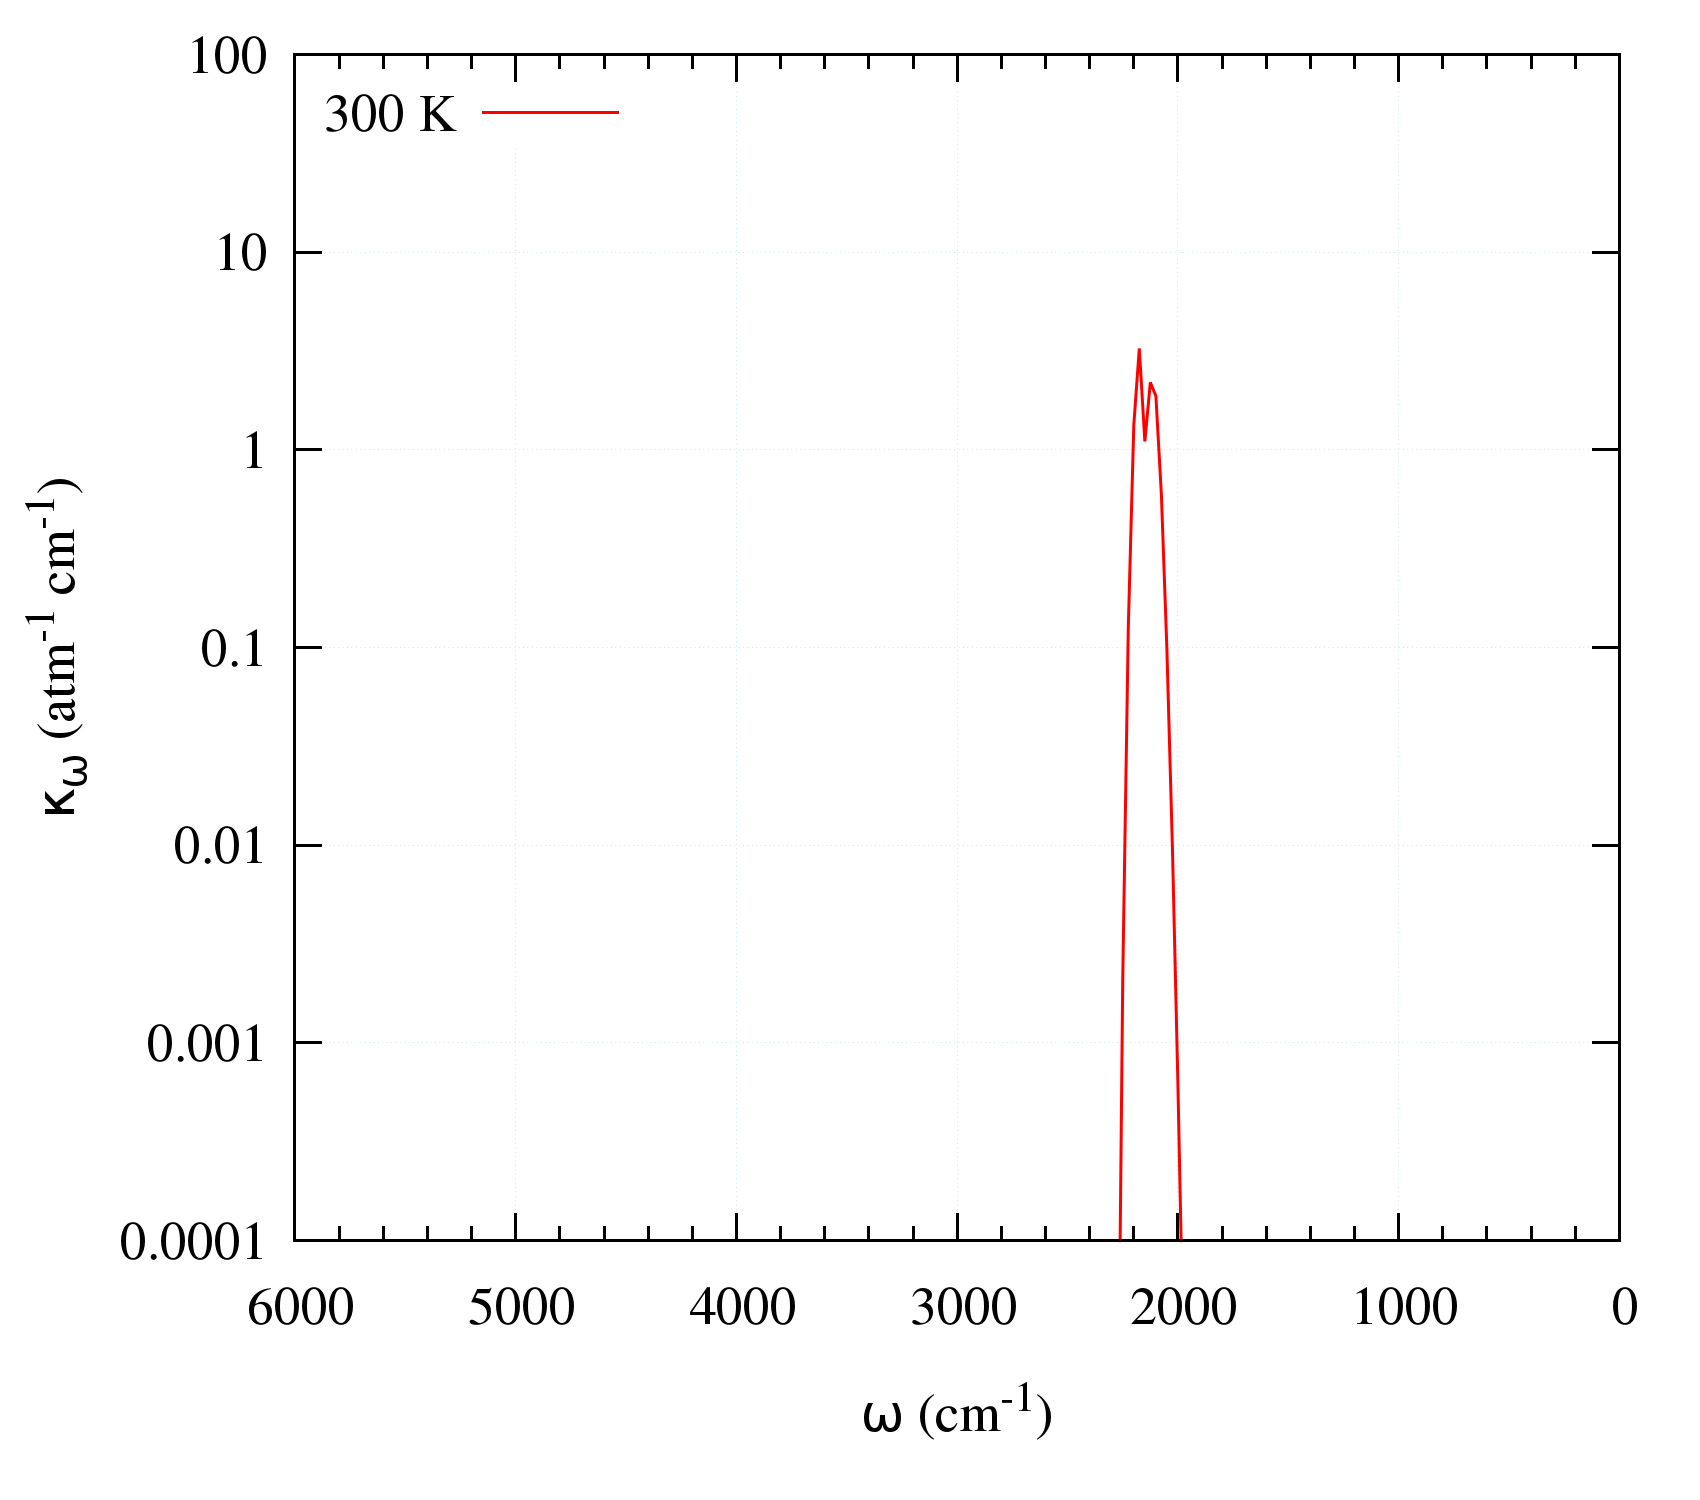
\includegraphics[height=2.5in]{Figures/CO_300K.png} &
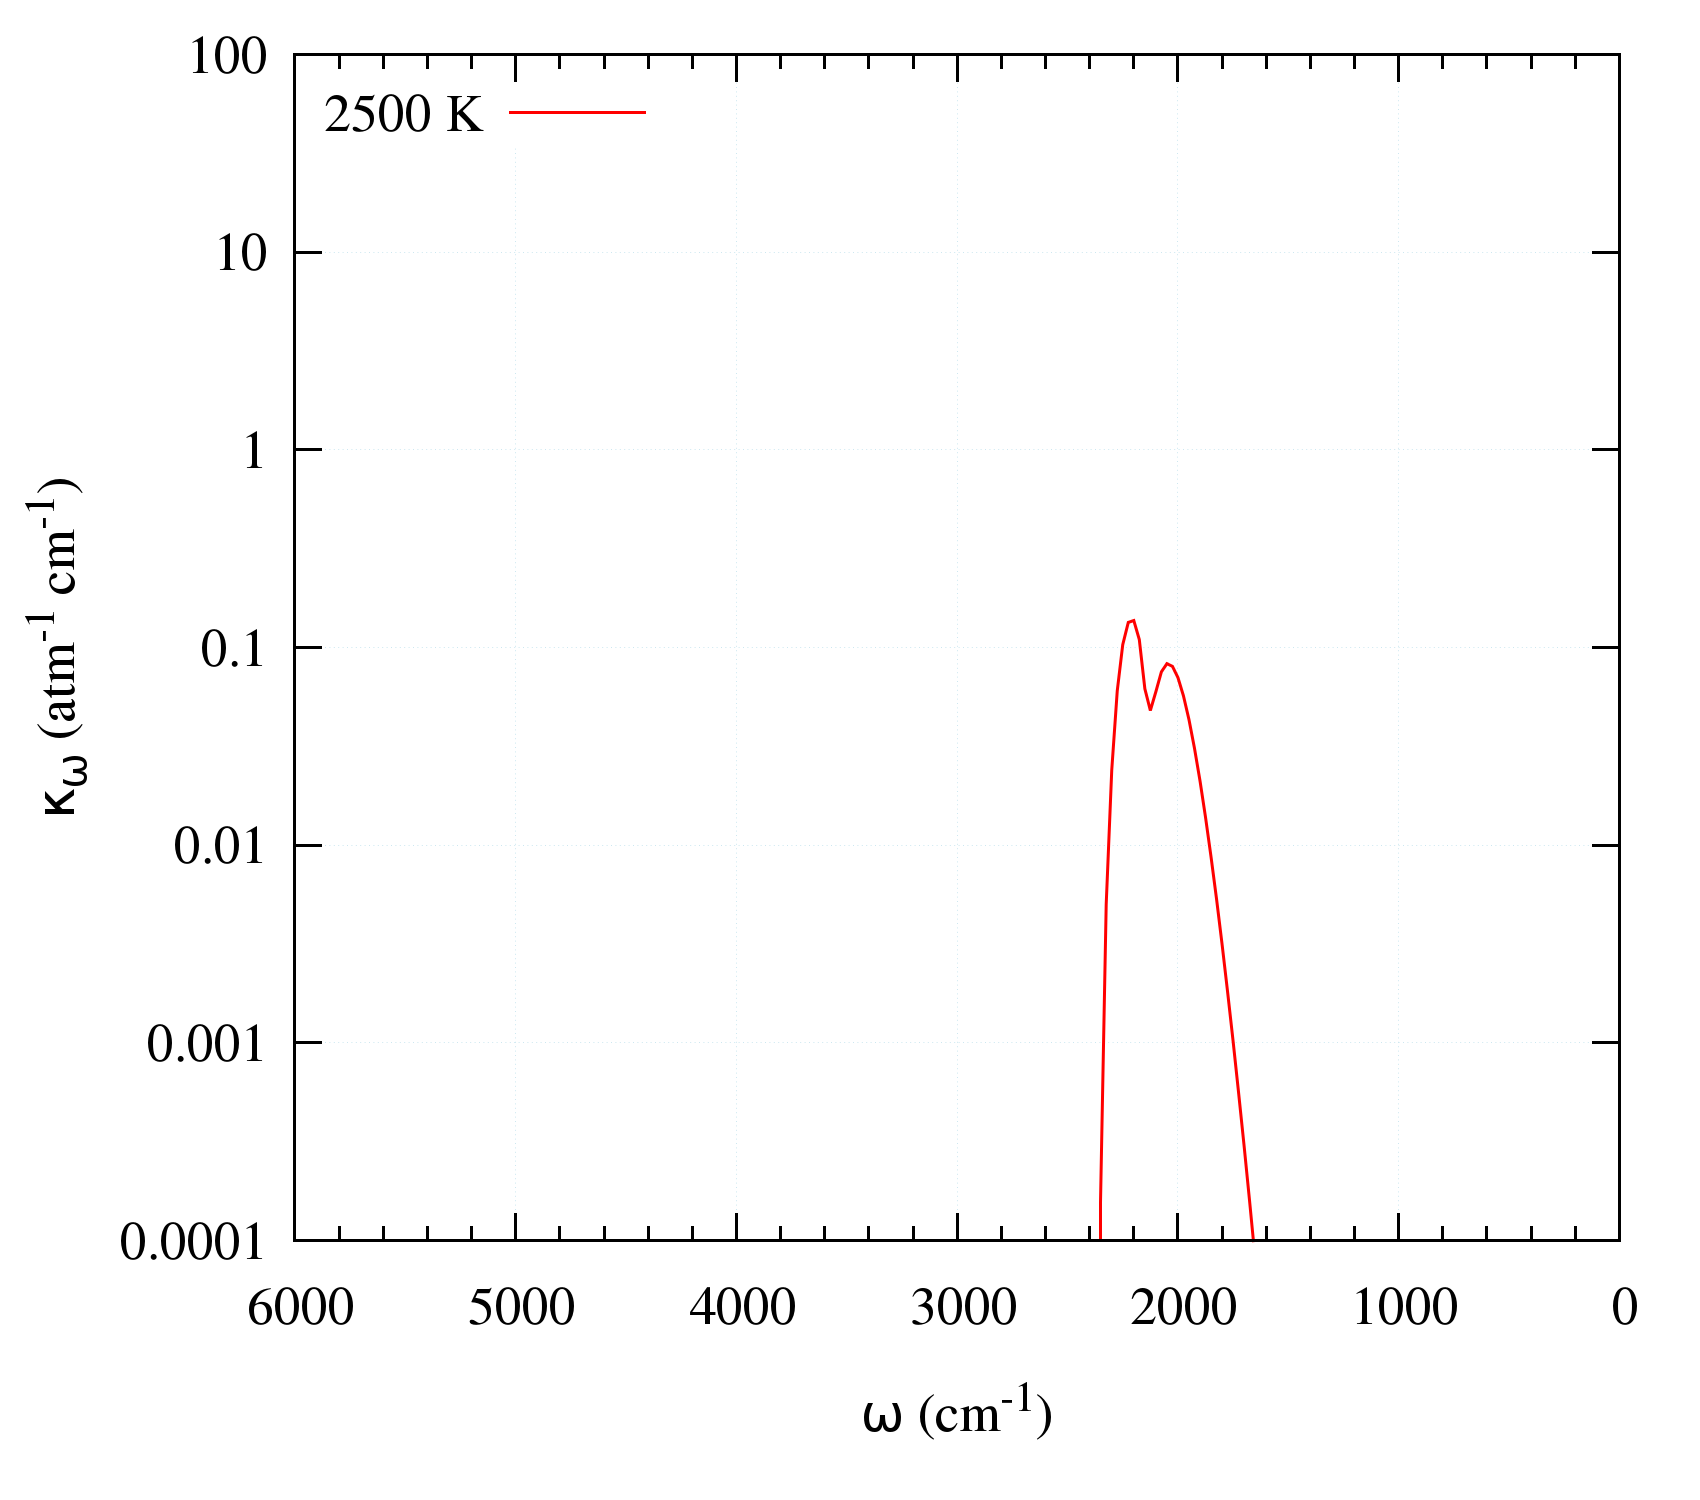
\includegraphics[height=2.5in]{Figures/CO_2500K.png} 
\end{tabular*}
\caption{Spectral variations of the CO mean absorption coefficient $\bar{\kappa}_{\om}$, in $\rm atm^{-1}.cm^{-1}$, at 300~K and 2500~K as tabulated in RadCal.\label{fig:CO_300-2500K}}
\end{figure}

The first overtone (centered at $ \om\approx 4260\;\rm {cm^{-1}}$) is not accounted for as its integrated band intensity is negligible at standard temperature and pressure. See Table \ref{Table::CO}. At 295~K, the integrated band intensity of Band~1 is $260\;\rm {atm^{-1}cm^{-2}}$. The statistical narrow band model associated with $\rm CO$ is the Goody model. Recommended temperatures of use range from 295~K to 2500~K.

\begin{table}[ht]
      \centering
      \caption{Spectral bands of $\rm CO$ included in RadCal.}
      \label{Table::CO}
    \begin{tabular}{|c|c|c|c|c|c|}
    \hline
    Band \# & \multicolumn{2}{|l|}{Bounds (cm$\rm ^{-1}$) } & Method & Assignment & $\alpha(T=296 \; {\rm K}) \; (\rm {atm^{-1} cm^{-2}})$   \\
    \cline{1-6}
    1 & 1600 & 2400 & modeled &  $\rm C\equiv O$ stretching & 260  \\
    \hline
   \end{tabular}
\end{table}


\clearpage

\section{Methane: $\rm CH_4$}

Methane is a spherical top molecule of tetrahedral shape with the carbon atom occupying the center of the tetrahedron. It belongs to the point group $T_d$. The methane IR spectrum is the result of the vibration-rotation modes of the $\rm C-H$ groups. It has nine vibrational modes, but due to its symmetry, this translates into only two distinct IR active fundamental vibration frequencies. In RadCal, the methane IR spectrum is divided into three distinct bands, which include the fundamentals plus degenerate (overtone) vibration modes. Bands 1 and 2 are calculated using tabulated mean absorption coefficient data which were obtained by Brosmer and Tien, \cite{Brosmer1985} for temperatures of 290, 600, 850~K. Band 3 is modeled, using a just-overlapping line model; the integrated intensities are computed in the harmonic-oscillator, rigid-rotator approximation. See Penner and Gray, Ref.~\cite{Gray1965}, for more details. In RadCal, the Elsasser model is used to calculate the collision optical depth. Table \ref{Table::CH4} tabulates the different characteristics of the $\rm CH_4$ bands.

\begin{table}[ht]
      \centering
      \caption{Spectral bands of $\rm CH_4$ included in RadCal.}
      \label{Table::CH4}
    \begin{tabular}{|c|c|c|c|c|c|}
    \hline
    Band \# & \multicolumn{2}{|l|}{Bounds (cm$\rm ^{-1}$) } & Method & Assignment & $\alpha(T=296 \; {\rm K}) \; (\rm {atm^{-1} cm^{-2}})$   \\
    \cline{1-6}
    1 & 1150 & 1600 & tabulated &  $\rm C-H$ Bend    & 237  \\
    2 & 2700 & 3250 & tabulated &  $\rm C-H$ Stretch & 212  \\
    3 & 3400 & 5000 & modeled   &  $\rm C-H$ Stretch &  35  \\
    \hline
   \end{tabular}
\end{table}
The strongest bands are Bands~1 and 2 which at standard temperature and pressure have an integrated band intensity of $237\;\rm {atm^{-1}cm^{-2}}$ and $212\;\rm {atm^{-1}cm^{-2}}$, respectively. Figure~\ref{fig:CH4_290-850K} displays the spectral mean absorption coefficient $\bar{\kappa}$ for $\rm CH_4$ at 290~K, 600~K, and 850~K, respectively.

\begin{figure}[ht]
\begin{tabular*}{\textwidth}{l@{\extracolsep{\fill}}r}
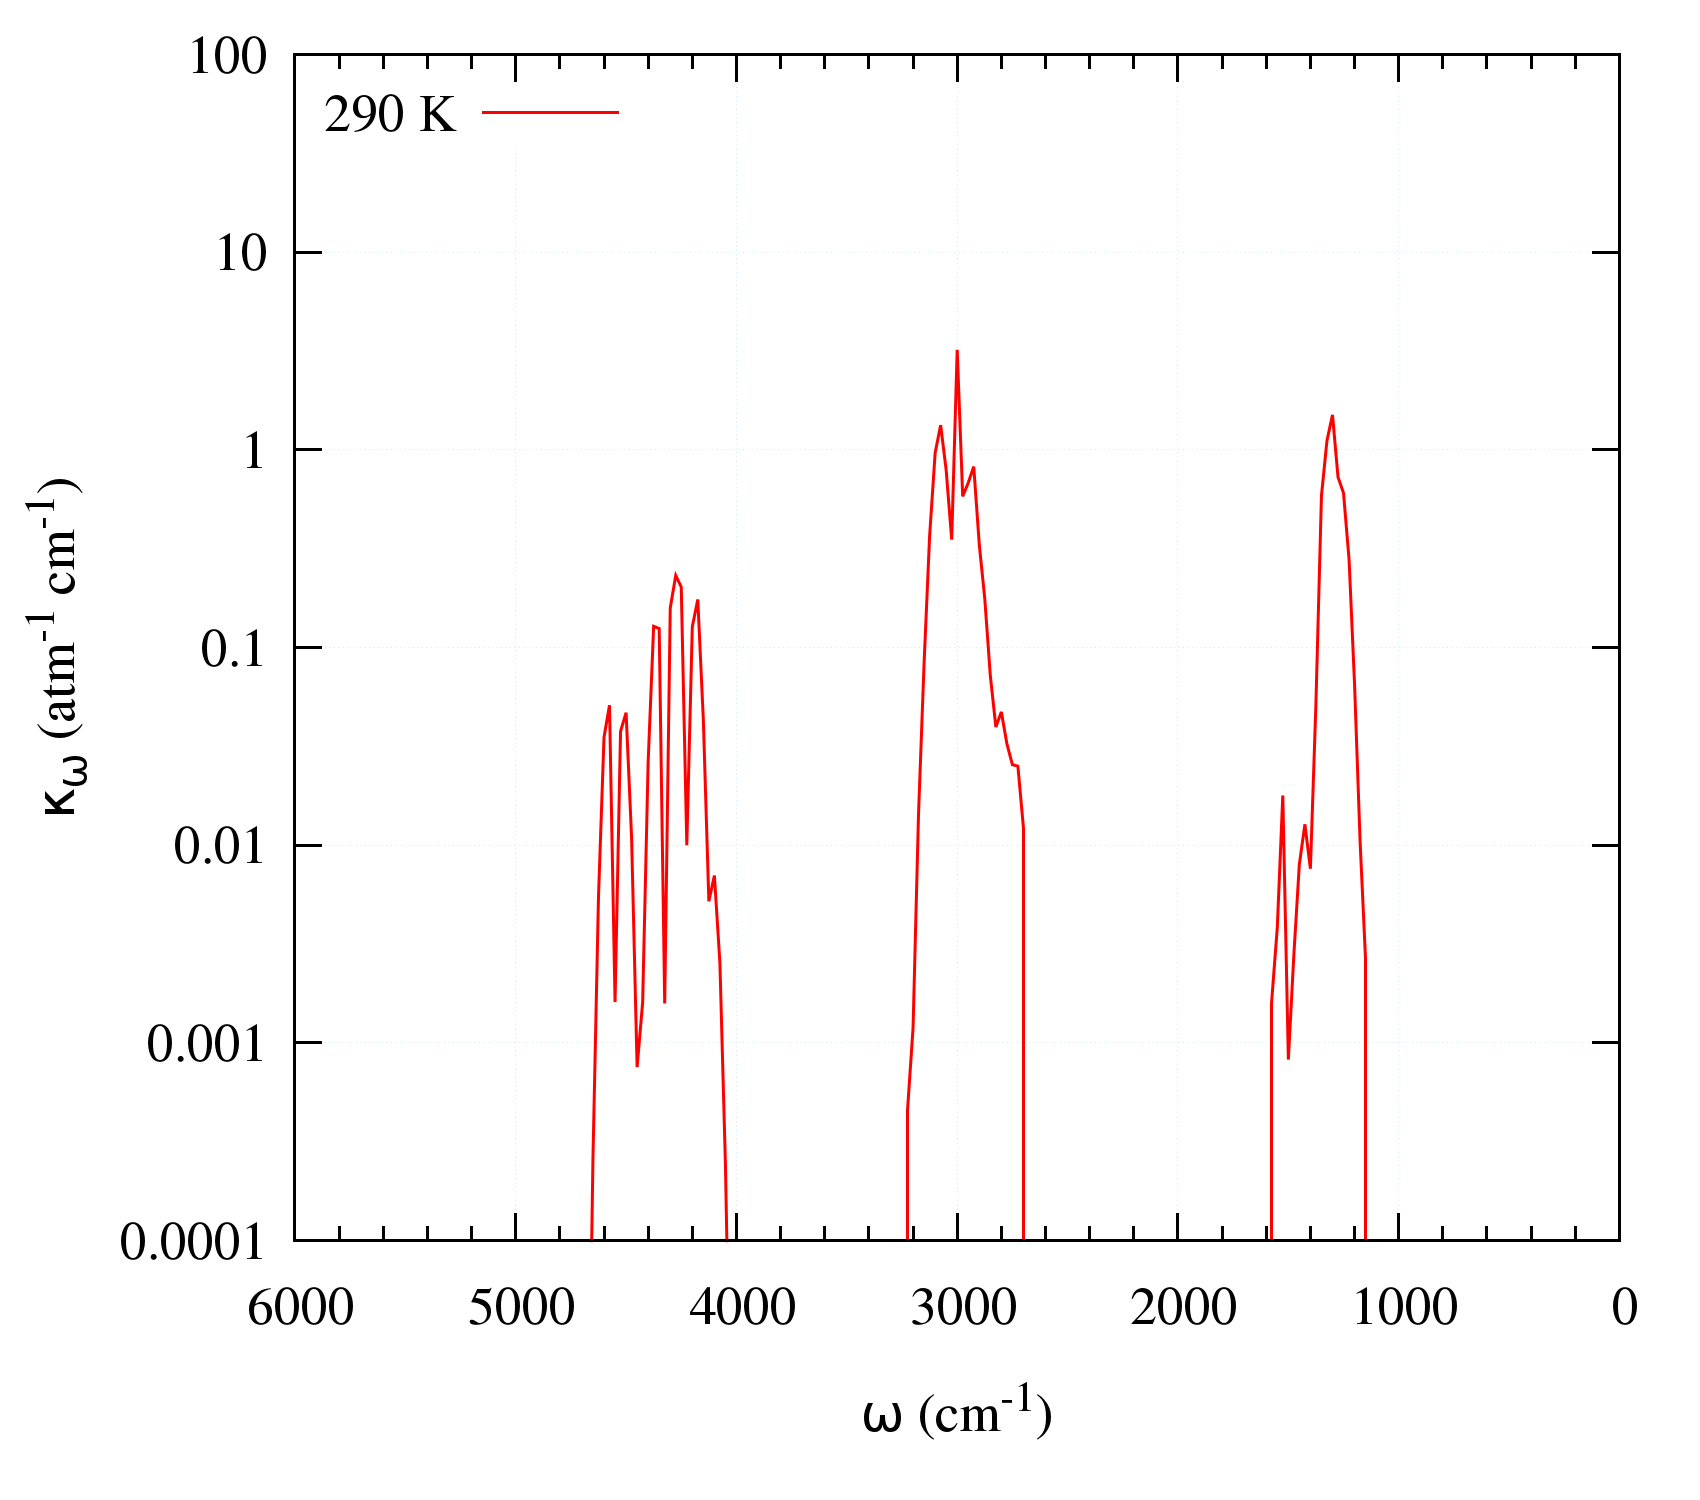
\includegraphics[height=2.5in]{Figures/CH4_290K.png} &
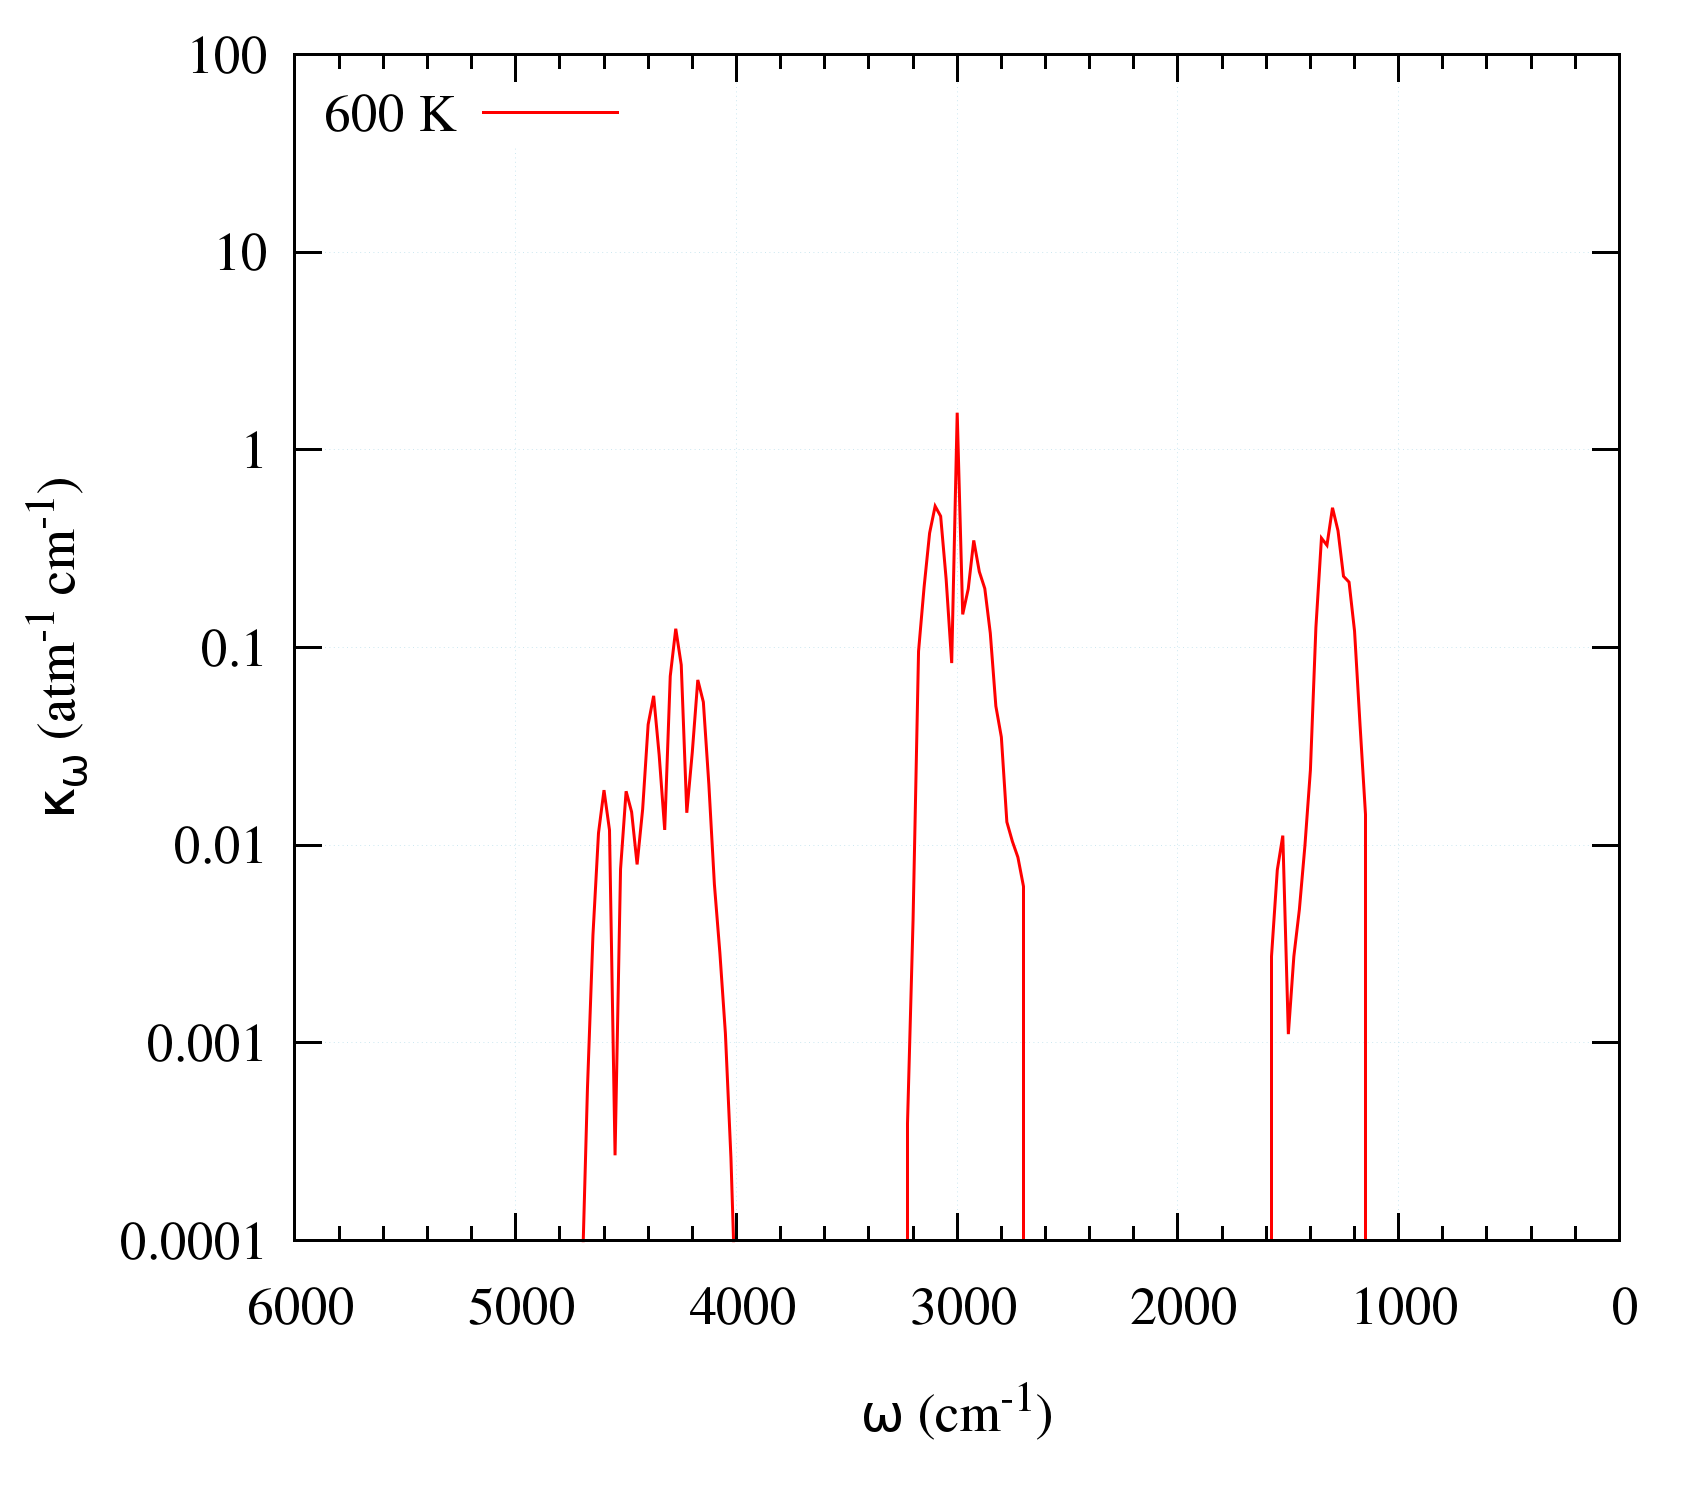
\includegraphics[height=2.5in]{Figures/CH4_600K.png} \\
\multicolumn{2}{c}{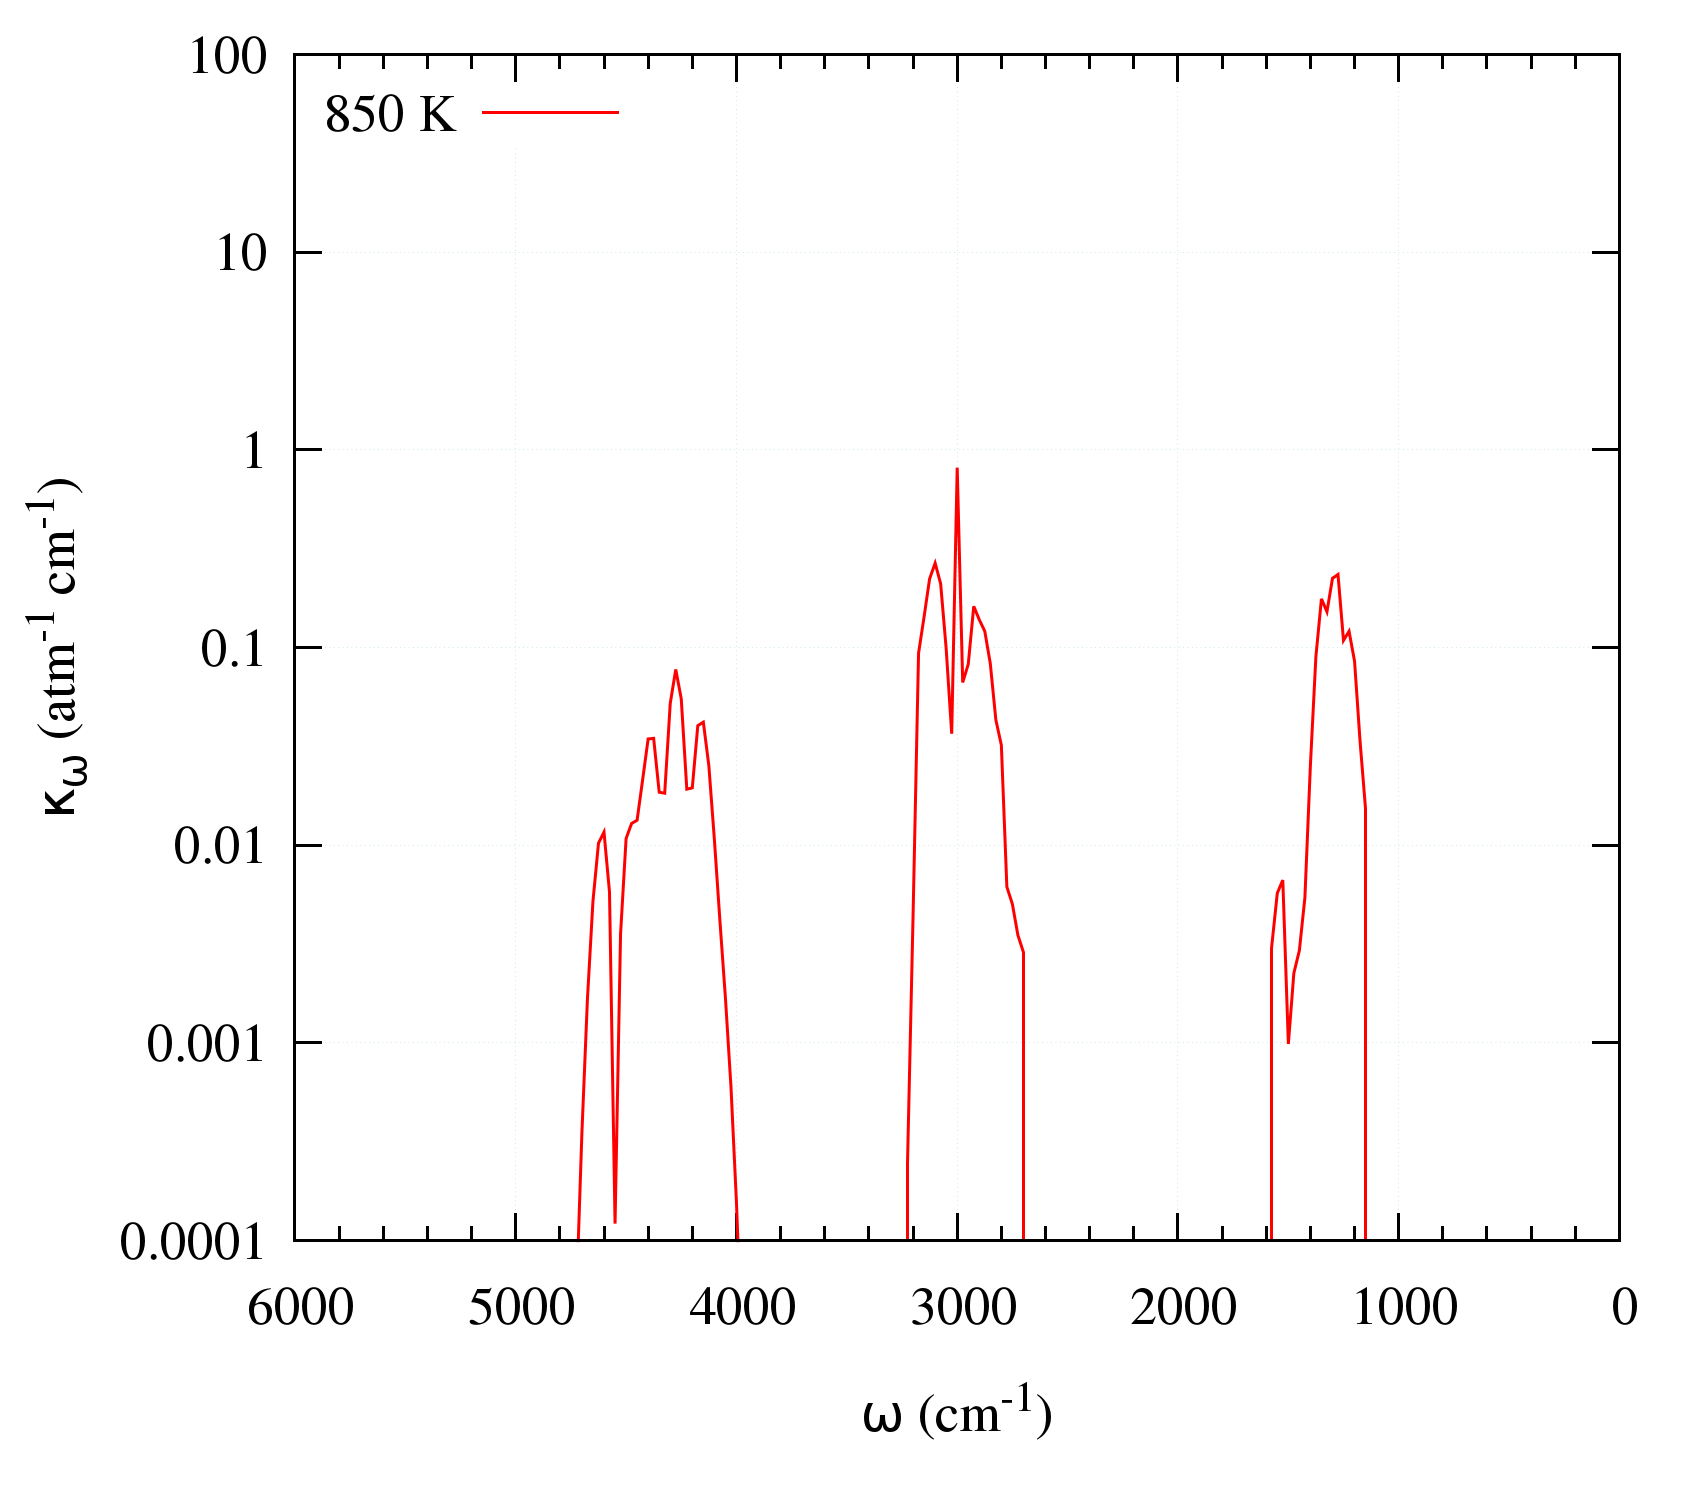
\includegraphics[height=2.5in]{Figures/CH4_850K.png}}
\end{tabular*}
\caption{Spectral variations of the $\rm CH_4$ mean absorption coefficient $\bar{\kappa}_{\om}$, in $\rm atm^{-1}.cm^{-1}$, at various temperatures as tabulated in RadCal.\label{fig:CH4_290-850K}}
\end{figure}

\clearpage

\section{Soot}

The soot spectral absorption coefficient is calculated using the below formulation:
\be\label{eq:soot_kappa}
\bar{\kappa} = 7.0 \om f_v
\ee
where $f_v$ is the soot volume fraction and is dimensionless. The narrow band transmissivity of soot is calculated as:
\be\label{eq::soot_optical_depth}
\bar{\tau}(0 \rightarrow s) = \exp\left(-\bar{\kappa} s \right).
\ee
From Eq.~\ref{eq:soot_kappa}, it can be seen that particulate matters tend to absorb soot in the high wavenumber part of the spectrum. Figure~\ref{fig:SOOT_300K} plots the spectral transmissivity of a homogeneous layer of soot at 300~K with a soot volume fraction value of 5~ppm ($5\times 10^{-6}$) and a thickness of 20~cm.

\begin{figure}[ht]
\begin{center}
 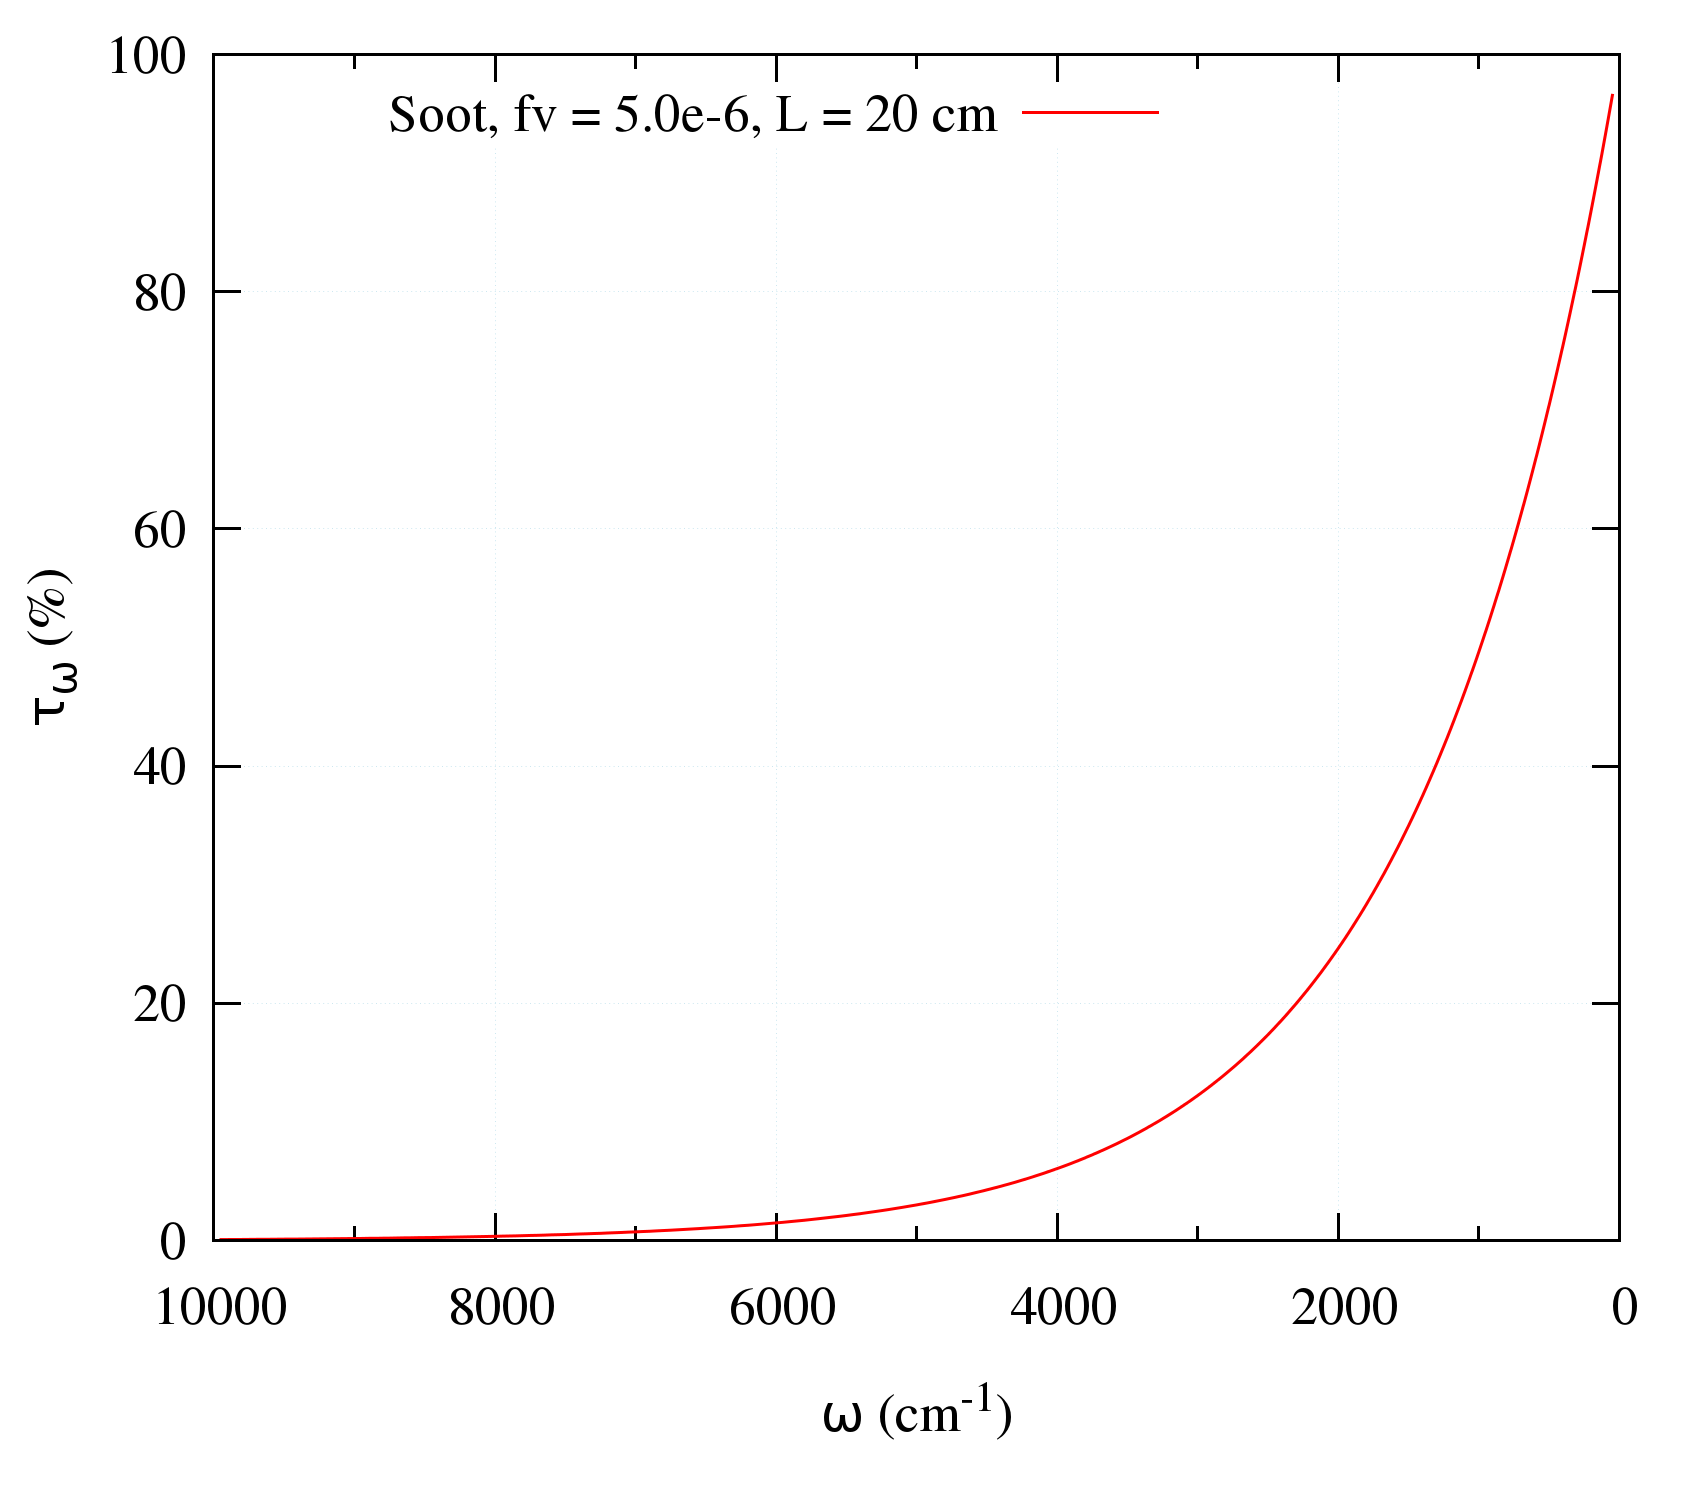
\includegraphics[height=2.5in]{Figures/SOOT_300K.png}
\end{center}
\caption{Predicted spectral transmissivity of a homogeneous layer of soot at 300~K, of thickness 20~cm, and with a soot volume fraction of 5~ppm ($f_v = 5\times 10^{-6}$).\label{fig:SOOT_300K}}
\end{figure}
